\chapter{Modeling}
\label{cha:Modeling}

To investigate the performance of the proposed cascade systems, mechanism models of the systems were developed with EES (Engineering Equation Solver) and MATLAB. Bottom-up design method was used for the system modeling. Firstly, the mechanism models developed in EES are used to validate the theoretical relationships of the models. Secondly, the component models were developed in MATLAB by using object-oriented method. It makes full use of inheritance and polymorphism to ensure both the independence and the relevance of the components.
%The cascade system is developed in several blocks. These blocks are made of circuits with efficiency calculations. 
Three circuits, air circuit, water circuit and oil circuit, were developed with some specific state parameters in some key components. Energy-based models of these key components were created on the basis of their thermodynamic behavior, heat transfer and the second law.

The following parts introduce models of some key components.
\section{Component modeling}
\subsection{Parabolic trough collector}
\label{sec:ptc}

%此部分需要细化

Parabolic trough collector consists of a reflector and a receiver. The reflector (mirror) reflects direct solar radiation and concentrates it onto a receiver tube located in the focal line of the parabola. The receiver is typically a metal absorber tube with high absorption rate coating. An outer glass tube is used outside the absorber tube to reduce thermal losses and the space between the absorber tube and the glass tube is usually drawn into a vacuum to further reduce the thermal losses.

Optical loss exists in the reflection process due to optical efficiency terms. The reflection terms can be listed as bellow~\cite{Price2002}:

\begin{itemize}
  \item Shadowing factor
  \item Tracking error
  \item Geometry error
  \item Clean mirror reflectance
  \item Dirt on mirrors
  \item Unaccounted errors
\end{itemize}

Another term, incident angle modifier $K(\theta)$, should be concerned when the solar irradiation is not normal to the collector aperture. It is a function of the solar incidence angle to the normal of the collector aperture ($\theta$).

The equation was determined from trough collector testing conducted at SNL~\cite{Dudley1994}.
\begin{equation}
  K(\theta) = \cos\theta+0.000884\theta-0.00005369\theta^2
\end{equation}

The optical losses are associated with five parameters (see Figure~\ref{fig:ParabolicTrough}):

\begin{enumerate}[label=(\arabic*)]
  \item Reflectivity, $\rho$: only a fraction of the incident radiation is reflected towards the receiver. The fraction is determined by the reflector type and dirt condition. Reflectivity of commercial parabolic trough mirrors can be assumed to be 0.9 for washed mirrors. 
  \item Intercept factor, $\gamma$: a fraction of the direct solar radiation reflected by the mirrors does not reach the glass cover of the absorber tube due to either microscopic imperfections of the reflectors or macroscopic shape errors in the parabolic trough concentrators (e.g., imprecision during assembly). These errors cause reflection of some rays at the wrong angle, and therefore they do not intercept the absorber tube. These losses are quantified by an optical parameter called the intercept factor, $\gamma$, that is typically 0.95 for a collector properly assembled.
  \item Transmissivity of the glass tube, $\tau$: only a fraction of the direct solar radiation reaching the glass cover of the absorber pipe is able to pass through it. The ratio between the radiation passing through the glass tube and the total incident radiation on it, gives transmissivity $\tau$,  which is typically 0.93.
  \item Absorptivity of the absorber selective coating, $\alpha_{abs}$: this parameter quantifies the amount of energy absorbed by the steel absorber pipe, compared with the total radiation reaching the outer wall of the steel pipe. This parameter is typically 0.95 for receiver pipes with a cermet coating, whereas it is slightly lower for pipes coated with black nickel or chrome.
  \item Soiling factor, $F_e$: because of the dirt on reflectors will reduce the reflectivity, it needs to concern the soiling factor. The soiling factor $F_e$ takes into account the progressive soiling of mirrors and glass tubes after washing.
\end{enumerate}

\begin{figure}[!ht]
\centering
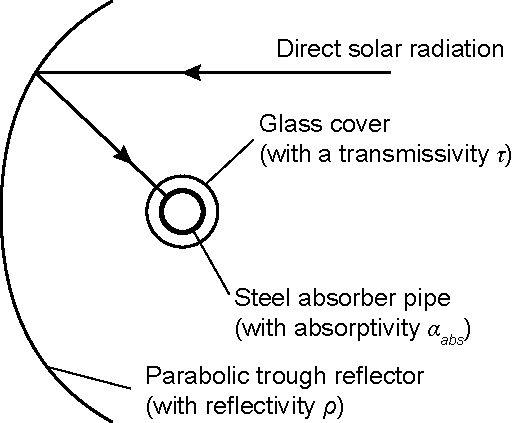
\includegraphics[width=0.4\textwidth]{fig/ParametersOfParablicDish.pdf}
\caption{Some of the optical parameters of a parabolic trough}\label{fig:ParabolicTrough}
\end{figure}

The energy pass through the glass tube to the receiver can be obtained by
\begin{equation}
  P = I_r w_{tc} L_{tc} \rho \gamma \tau F_e K(\theta)
\end{equation}

The solar energy absorbed by the absorber occurs very close to the outer surface, to simplify the absorption process, it is treated as a uniform heat flux $q''$.

\begin{equation}
  q''= \frac{P}{\pi d_o L_{tc}} = \frac{I_r w_{tc} \rho \gamma \tau F_e K(\theta)}{\pi d_o}
\end{equation}
%
%Yilmaz et al.~\cite{Yilmaz2014} 
%
%LUZ solar collector LS-3 is used as the trough collector.
%%For a trough collector, 
%The heat flux to the outer surface of the receiver can be obtained by $q''=I_rw_{tc}\eta_{opt,0}K(\phi)F_{e}/P$, where $P=\pi{}d_o$, $K(\phi)$ is the incidence angle modifier, $\eta_{opt,0} = \rho \gamma \tau \alpha_{abs}$
%is peak optical efficiency (optical efficiency with an incidence angle of 0).
%\nomenclature{$K$}{Incidence angle modifier of trough collector}
%%\nomenclature[G]{$\eta_{opt,0}$}{Optical efficiency with an incidence angle of 0}

Assume overall heat transfer coefficient $U(T_{abs})$ is uniform for whole length of the collector, and the heat transfer correlation in Appendix ~\ref{cha:CTCHFHX} can be used. Figure~\ref{fig:Pipe} shows the schematic diagram of the thermal analysis of the absorber pipe.
\nomenclature{$U$}{Overall heat transfer coefficient, W$\cdot$m$^{-2}\cdot$K$^{-1}$}
\nomenclature{$q''$}{Heat flux, W$\cdot$m$^{-2}$}
\begin{equation}
	\frac{T_{o}-T_{amb}-\dfrac{q''}{U(T_{abs})}}{T_{i}-T_{amb}-\dfrac{q''}{U(T_{abs})}}=\exp(-\frac{U(T_{abs})\pi d_o L_{tc}}{\dot{m}c_{p}})\label{eq:CTCHF}
\end{equation}

\begin{figure}[!ht]
\centering
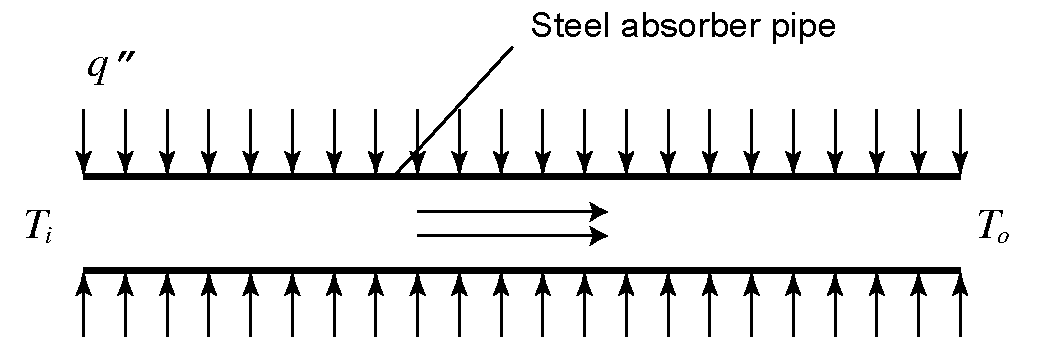
\includegraphics[width=0.6\textwidth]{fig/Pipe.pdf}
\caption{Schematic diagram of the absorber pipe}\label{fig:Pipe}
\end{figure}


Since the Nusselt number $Nu$ in the pipe is very large (about 1$\times$10$^4$), small temperature difference exists between the absorber and oil. So the average fluid temperature $(T_{i}+T_{o})/2$ can be used as the average value of $T_{abs}$, and $U(T_{abs})$ can be obtained by the a second-order polynomial function given by Romero and Zarza~\cite{Romero2007}. The length $L_{tc}$ required to get the required number of trough collectors in a row can be obtained from Equation~(\ref{eq:CTCHF}).

The energy projected perpendicularly to the aperture of the trough collectors is

\begin{equation}
  Q_{total} = I_r L_{tc} w_{tc}
\end{equation}

The energy absorbed by the heat transfer fluid is 

\begin{equation}
  Q_{use} = \dot{m}c_p(T_o - T_i)
\end{equation}

The thermal efficiency of the trough collectors 

\begin{equation}
  \eta_{tc} = \dfrac{Q_{use}}{Q_{total}} = 
  \dfrac{I_r L_{tc} w_{tc}}{\dot{m}c_p(T_o - T_i)}
  \label{eq:eta_tc}
\end{equation}

\subsection{Parabolic dish collector}
\label{sec:pdc}

Parabolic dish collector consists of a reflector and a receiver. The reflector (mirror) tracks the sun to reflect direct solar radiation and concentrates it onto a receiver located at the focal point of the reflector. Two axes tracking system needs to be applied for the reflector to continuously follow the daily path of the sun.

Two different methods~\cite{Adkins1987} are applied for the sun tracking systems:
\begin{itemize}
  \item Azimuth elevation tracking by an orientation sensor or by calculated coordinates of the sun performed by the local control.
  \item Polar tracking, where the concentrator rotates about an axis parallel to the earth’s axis rotation.
\end{itemize}

In a traditional dish-Stirling system, a Stirling engine is located at the focal point. The Stirling engine has a receiver to absorb the thermal energy from the concentrated sunlights. The receiver consists of an aperture and an absorber. The aperture in a Stirling receiver is located at the focal point of the reflector to reduce the radiation and convection losses. The absorber absorbs the solar radiation and transfers the thermal energy to the working gas of the Stirling engine. An electrical generator, directly connected to the crankshaft of the engine, converts the mechanical energy into electricity. 

In the proposed cascade system, a volumetric receiver is located on the focal point. Spiral tube is located in the receiver to absorb the concentrated solar energy. Air (or nitrogen, is used as the heat transfer fluid) flows trough the tube to transfer the absorbed energy as the heat source of Stirling engine(s).

The reflector is a key element of the systems. The curved reflective surface can be manufactured by attached segments, by individual facets or by a stretched membranes shaped by a continuous plenum. In all cases, the curved surface should be coated or covered by aluminum or silver reflectors. 

A dish reflector product of SES (Stirling Energy System) is used in this cascade system, and its key parameters can be found in Table~\ref{tab:dc}. The structure of the receiver is shown in Figure~\ref{fig:dishReceiver}.

\begin{figure}[!ht]
\centering
\includegraphics[width=0.6\textwidth]{fig/DishReceiver.pdf}
\caption{The structure of the dish receiver}\label{fig:dishReceiver}
\end{figure}

\begin{table}[htbp]
	\caption{Key parameters of the dish collector}
	\begin{center}
	\begin{tabular}{cccccc}
		\toprule
		Parameter		&	Value	&	Parameter		&	Value	&	Parameter		&	Value\\
		\midrule
		$d_{cav}$	&	0.46$\,\mathrm{m}$	&	$\epsilon_{insu}$	&	0.6	&	$\theta_{dc}$	&	45$^\circ$\\
		$\delta_{insu}$	&	0.075$\,\mathrm{m}$	&	$\alpha_{cav}$	&	0.87	&	$\gamma$	&	0.97\\
		$dep_{cav}$	&	0.23$\,\mathrm{m}$	&	$\delta_a$		&	0.005$\,\mathrm{m}$	&	$\eta_{shading}$	&	0.95\\
		$d_{ap}$	&	0.184$\,\mathrm{m}$	&	$d_{i,1}$	&	0.07$\,\mathrm{m}$	&	$\rho$	&	0.91\\
		$\lambda_{insu}$	&	0.06$\,\mathrm{W/(m\cdot K)}$	&	$A_{dc}$	&	87.7$\,\mathrm{m^2}$	&	\\		
		\bottomrule
	\end{tabular}
	\end{center}
	\label{tab:dc}
\end{table}
\nomenclature[G]{$\delta$}{Thickness, m}
\nomenclature[S]{$insu$}{Insulating layer}
%\nomenclature[G]{$\delta_{insu}$}{Thickness of receiver insulating layer, m}
\nomenclature{$dep$}{Depth, m}
\nomenclature{$d$}{Diameter, m}
\nomenclature[G]{$\lambda$}{Thermal conductivity, W$\cdot{}$m$^{-1}$$\cdot$K$^{-1}$}
\nomenclature[G]{$\epsilon$}{Emissivity}
%\nomenclature[G]{$\lambda_{insu}$}{Thermal conductivity of receiver insulating layer, $\mathrm{W/(m\cdot K)}$}
%\nomenclature[G]{$\epsilon_{insu}$}{Emissivity of reciver insulating layer}
%\nomenclature[G]{$\delta_{a}$}{Thickness of air tube in volumetric receiver, m}
%\nomenclature{$d_{i,1}$}{Inner diameter of air tube, m}
\nomenclature[G]{$\theta_{dc}$}{Dish aperture angle (0$^{\circ}$ is horizontal, 90$^{\circ}$ is vertically down)}
\nomenclature[G]{$\gamma$}{Intercept factor; compression ratio}
\nomenclature[G]{$\eta_{shading}$}{Shading factor}
\nomenclature[G]{$\rho$}{Reflectivity}
\nomenclature{$A_{se,1}$}{Heat transfer area of Stirling engine at air side, m$^2$}
\nomenclature{$A_{se,2}$}{Heat transfer area of Stirling engine at water side, m$^2$}
%\nomenclature{$k$}{Specific heat ratio}
%\nomenclature[G]{$\gamma_{se}$}{Compression ratio of Stirling engine}
\nomenclature{$n_g$}{Amount of working gas in each Stirling engine, mol}
\nomenclature{$n_{se}$}{Number of Stirling engines in the Stirling engine array}

The dish receiver model concerns the losses include: collector losses due to mirror reflectivity, receiver intercept losses, losses due to shading, and thermal losses. Thermal losses take the largest portion of all those losses, which are due to conduction, convection and radiation. Figure~\ref{fig:thermal-lose} shows the thermal network of dish receiver, which concerns the losses:
\begin{itemize}
	\item Radiation losses reflected off of the receiver cavity surfaces and out of the receiver through the aperture. ($q_{rad,ref}$)
	\item Conductive losses through the receiver insulating layer. ($q_{cond,tot}$)
	\item Free convection from the cavity in the absence of wind. ($q_{conv,free}$)
	\item Forced convection in the presence of wind. ($q_{conv,forc}$)
	\item Emission losses due to thermal radiation emitted from the receiver aperture. ($q_{rad,emit}$)
\end{itemize}

\noindent \begin{figure}[htbp]
\begin{center}
	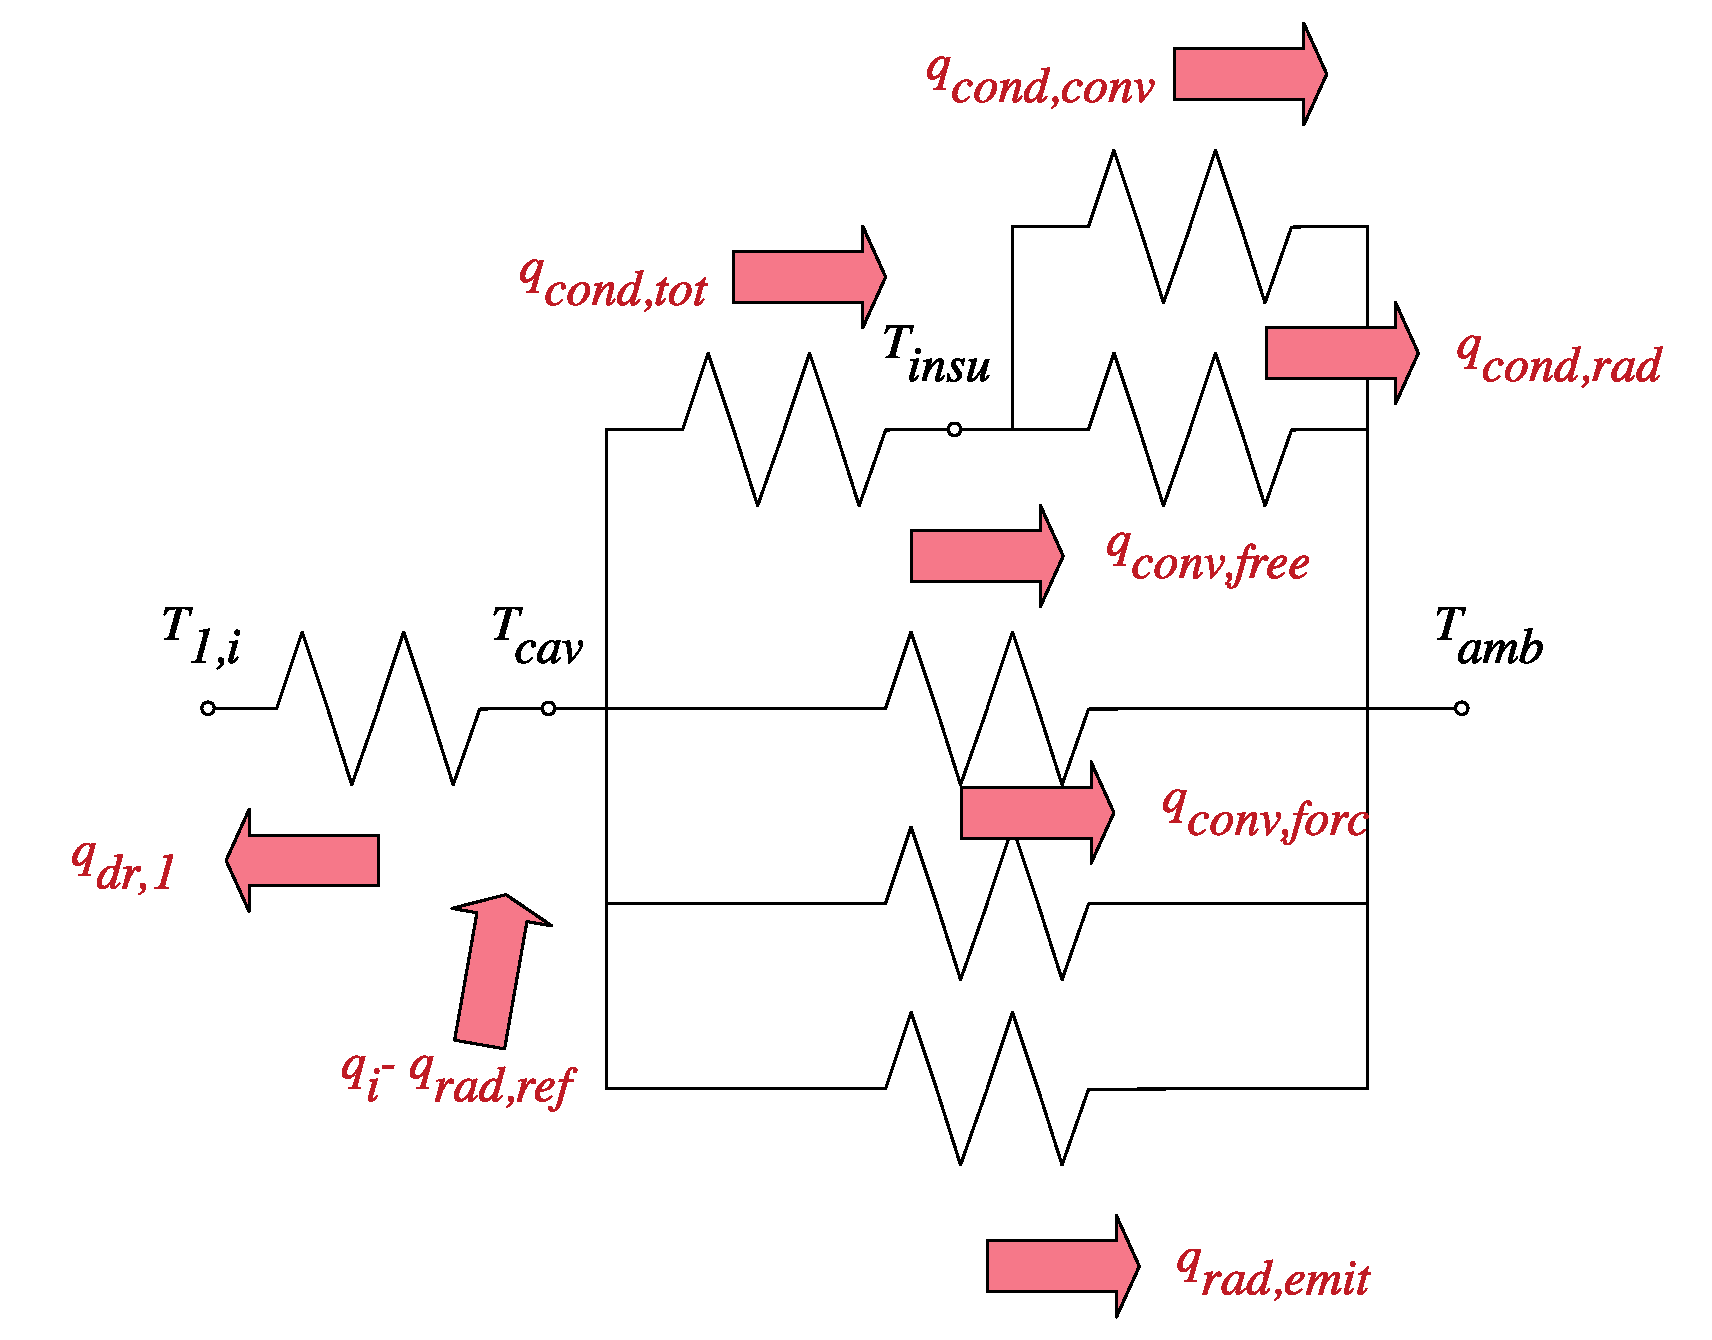
\includegraphics[width = 0.7\columnwidth]{fig/thermalLosses.pdf}
	\caption{Thermal network of dish receiver}
	\label{fig:thermal-lose}
\end{center}
\end{figure}

To solve the thermal network in Figure~\ref{fig:thermal-lose}, correlations and relationships of the heat fluxes should be clear.

\begin{enumerate}[label=(\arabic*)]
  \item \emph{Inlet energy from the reflector, $q_i$}
  
  To simplify the model, influences made by receiver blocking and imperfection track are ignored.  
  \begin{equation}
      q_i = I_r A_{dc} \gamma \eta_{shading} \rho
      \label{eq:q_i}
  \end{equation}
  
  In Equation~(\ref{eq:q_i}), $\gamma$ is the intercept factor, $\eta_{shading}$ is the shading factor between different collectors, $\rho$ is the reflectivity of the reflector.
  \item \emph{Heat exchange between the HTF and the dish absorber, $q_{dr,1}$}
  
  The heat transfer process between the HTF and the dish absorber is simplified to a heat exchange process of a flow in a uniform temperature heat pipe. So $q_{dr,1}$ can be written as  
  \begin{equation}
      q_{dr,1} = h_{dr,1}A_{dr,1}\Delta T_{ln,dr,1}
      \label{eq:q_dr_1}
  \end{equation}
  \nomenclature{$A_{dr,1}$}{Heat transfer area of dish receiver between tube and air, $\mathrm{m^2}$}  
  where  
  \begin{equation}
      h_{dr,1} = Nu_{tube}\lambda_{dr,1} / d_{i,1}
\end{equation}
\begin{equation}
      Nu_{tube} = c_r Nu'_{tube}
\end{equation}
    \nomenclature{$Nu$}{Nusselt number}
    \nomenclature{$c_r$}{Heat transfer correction factor of coiled tube of volumetric receiver}
    For helical spiral pipe, multiplier $c_r$ based on curvature ratio can be written as~\cite{Pablo2008}
\begin{equation}
	c_{r}=1+3.5\frac{d_{i,1}}{d_{cav}-d_{i,1}-2\delta_{a}}
\end{equation}
$Nu'_{tube}$ is the Nusselt number of straight circular tube, which can be obtained by~\cite{Serth2007}
\begin{equation}
	Nu'_{tube}= 0.027Re_{tube}^{0.8}Pr_{tube}^{1/3}(\mu_{tube}/\mu_{tube,w})^{0.14}
\end{equation}
\nomenclature{$Pr$}{Prandtl number}
\nomenclature{$Re$}{Reynolds number}
\nomenclature[G]{$\mu$}{Viscosity, kg$\cdot$m$^{-1}$$\cdot$s$^{-1}$}
\nomenclature[S]{$w$}{Tube wall}
and the logarithmic mean temperature difference $\Delta{}T_{ln,dr,1}$ can be written as
\begin{equation}
	\Delta{}T_{ln,dr,1}=\frac{(T_{cav}-T_{dc,i})-(T_{cav}-T_{dc,o})}{\ln\dfrac{T_{cav}-T_{dc,i}}{T_{cav}-T_{dc,o}}}
\end{equation}

  \item \emph{Radiation losses reflected off the receiver, $q_{rad,ref}$}
  \begin{equation}
    q_{rad,ref}=(1-\alpha_{eff})q_{i}
\end{equation}
    where $\alpha_{eff}$ is the effective absorptivity of the receiver.    
    \begin{equation}
    \alpha_{eff}=\frac{\alpha_{cav}}{\alpha_{cav}+(1-\alpha_{cav})\dfrac{A_{ap}}{A_{cav}}}
    \end{equation}
    
    $\alpha_{cav}$ is the absorptivity of the cavity, $A_{cav}$ is the cavity area, $A_{ap}$ is the aperture area.
  \item \emph{Conductive losses through the receiver insulating layer, $q_{cond,tot}$}
  
  \begin{equation}
q_{cond,tot}=2\pi\lambda_{insu}dep_{cav}\dfrac{T_{cav}-T_{insu}}{\ln((d_{cav}+2\delta_{insu})/d_{cav})}
    \end{equation}
    
    where $T_{cav}$ is the temperature of the cavity wall, $T_{insu}$
is outside temperature of the insulation wall.

  \item \emph{Convection losses from the receiver insulating layer, $q_{cond,conv}$}  
  \begin{equation}
%\begin{split}
	q_{cond,conv}=h_{insu}A_{insu}(T_{insu}-T_{amb})
	=\dfrac{k_{insu}Nu_{insu}A_{insu}(T_{insu}-T_{amb})}{d_{cav}+2\delta_{insu}}
%\end{split}
\end{equation}
%\nomenclature{$k_{insu}$}{Thermal conductivity of air at the temperature of outside insulating layer, W$\cdot$m$^{-1}\cdot$K$^{-1}$}
where $Nu_{insu}$ can be obtained by the correlation for flow over a circular cylinder.~\cite{Churchill1977}

  \item \emph{Radiation losses from the receiver insulating layer, $q_{cond,rad}$}  
  \begin{equation}
	q_{cond,rad}=\epsilon_{insu}A_{insu}\sigma(T_{insu}^4 - T_{amb}^4)
\end{equation}
  \item \emph{Free convection from the cavity in the absence of wind, $q_{conv,free}$}
    
  Ma~\cite{Ma1993} conducted tests to determine the free convection losses from the receiver for alternative setups, and the data were consistent with Stine and McDonald's free convection correlation. It is assumed that forced convection is independent of free convection in the receiver, so the total convection losses can be represented as the total of the free and forced convection losses as shown in Figure~\ref{fig:thermal-lose}.  
  \begin{equation}
	q_{conv,free} = h_{free}A_{cav}(T_{cav}-T_{amb})
\end{equation}
where $h_{free}=k_{film}Nu_{free}/\overline{d_{cav}}$, $\overline{d_{cav}}$ is the effective diameter of the cavity, $\overline{d_{cav}}=d_{cav}-2d_i-4 \delta_a$.
\nomenclature{$\overline{d_{cav}}$}{Effective diameter of the cavity, m}
\nomenclature{$d_i$}{Inner diameter of trough receiver, m}$d_{i}=$0.066$\,$m
  
  \item \emph{Force convection from the cavity in the presence of wind, $q_{conv,forc}$}  
  \begin{equation}
	q_{conv,forc} = h_{forc}A_{cav}(T_{cav}-T_{amb})
\end{equation}

    Wu et al.~\cite{Wu2010} present a comprehensive review and systematic summarization of convection heat loss from cavity receiver in parabolic dish solar thermal power system. And we choose the correlation presented by Leibfried and Ortjohann~\cite{Leibfried1995}. This correlation gives an extended model of Koenig and Marvin~\cite{Koenig1981} and Stine and Diver~\cite{Stine1994} with better results.

For forced convection loss, side-on wind convection loss model given by Ma~\cite{Ma1993}, which is independent of the aperture orientation, is used
\begin{equation}
	h_{forc}=0.1967v_{wind}^{1.849}
\end{equation}

  \item \emph{Emission losses due to thermal radiation emitted from the receiver aperture, $q_{rad,emit}$}
  
  The emissivity is set equal to the effective absorptivity of the cavity (gray body),
\begin{equation}
    \epsilon_{cav}=\alpha_{eff}
\end{equation}
\begin{equation}
    q_{rad,emit}=\epsilon_{cav}A_{ap}\sigma(T_{cav}^{4}-T_{amb}^{4})
\end{equation}
\end{enumerate}

From Figure\ref{fig:thermal-lose}, it can be found that

\begin{equation}
  q_{eff} = q_i - q_{rad,ref}
\end{equation}
\begin{equation}
  q_{eff} = q_{dr,1} + q_{cond,tot} + q_{conv,free} + q_{conv,forc}+q_{rad,emit}
\end{equation}
\begin{equation}
  q_{cond,tot} = q_{cond,conv}+q_{cond,rad}
\end{equation}

So the temperature nodes in the thermal network can be solved by these equations.

$q_{dr,1}$ can be obtained by Equation~(\ref{eq:q_dr_1}), and efficiency of the dish receiver
\begin{equation}
  \eta_{dr} = \frac{q_{dr,1}}{q_i}
\end{equation}

Efficiency of the dish collector
\begin{equation}
  \eta_{dc} = \frac{q_{dr,1}}{I_rA_{dc}}
\end{equation}

\subsection{Stirling engine}\label{sec:StirlingEngineModel}
\subsubsection{Theoretical Stirling cycle}
In a Stirling cycle, there are two isothermal processes that exchange heat with heating and cooling fluids, two isochoric processes that exchange heat with regenerator. In Figure~\ref{fig:StirlingCycle}, the heat absorbed by regenerator in process 4-1 is reused in process 2-3, but only able to heat the working gas from 2 to 3' due to the imperfect regeneration. $e$ is defined as the regenerator effectiveness\cite{Formosa2010,Juhasz2010}, $e=\frac{T_R-T_L}{T_H-T_L}$, where $T_H$ is the temperature in the hot space, $T_L$ is the temperature in the cold space, $T_R$ is the effective working fluid temperature in the regenerator.
\nomenclature{$e$}{Regenerator effectiveness}
\nomenclature{$T_R$}{Effective working fluid temperature in regenerator, K}
\nomenclature{$T_L$}{Working fluid temperature in the cold space, K}
\nomenclature{$T_H$}{Working fluid temperature in the hot space, K}

\noindent \begin{figure}[htbp]
\begin{center}
	\includegraphics[width = 0.7\columnwidth]{fig/StirlingCycle}
	\caption{$T$-$s$ diagram of a Stirling cycle}
	\label{fig:StirlingCycle}
\end{center}
\end{figure}

In order to obtain a simplified analytical model, several simplifications were made:

\begin{itemize}
\item The working gas in Stirling engines obeys the idea gas law.
\item No heat loss to the environment for Stirling engines.
\item Overall heat transfer coefficients of the fluids are constant.
\item A symmetrical regenerator behavior is assumed~\cite{Formosa2010,Juhasz2010} so that a simple effectiveness can be obtain by $T_{R}=\frac{T_{H}-T_{L}}{\ln(T_{H}/T_{L})}$.
\end{itemize}

To consider internal irreversibilities in Stirling cycle made by dead volumes, total dead volume $V_D$ can be divided into heater dead volume $V_{DH}$, regenerator dead volume $V_{DR}$ and cooler dead volume $V_{DC}$.~\cite{Duan2014}, There exists a factor $K$ to describe the dead volumes under different temperatures. $K$ is relevant with temperatures in the process and regenerator effectiveness.
\nomenclature{$V_D$}{Total dead volume, m$^3$}
\nomenclature{$V_{DH}$}{Hot space dead volume, m$^3$}
\nomenclature{$V_{DR}$}{Regenerator dead volume, m$^3$}
\nomenclature{$V_{DC}$}{Cold space dead volume, m$^3$}
\begin{equation}
	K = \frac{V_{DH}}{T_H} + \frac{V_{DR}}{T_R} + \frac{V_{DC}}{T_L}
\end{equation}
\nomenclature{$K$}{Dead volume factor}

For the isothermal compression process 1-2, the output work
\begin{equation}
	W_{12} = \int^{V_E}_{V_E+V_C}{p_{12}dV}=-mRT_L\ln{\frac{V_E+V_C+KT_L}{V_E+KT_L}}
\end{equation}
%\nomenclature{$W_{12}$}{Output work in process 1-2 (J)}
\nomenclature{$V_E$}{Expansion volume, m$^3$}
\nomenclature{$V_C$}{Compression volume, m$^3$}
\nomenclature{$m$}{Mass of working fluid in Stirling engine, kg}
\nomenclature{$R$}{Gas constant, J$\cdot$kg$^{-1}\cdot$K$^{-1}$}

For the isothermal expansion process 3-4, the output work
\begin{equation}
	W_{34} = \int^{V_E+V_C}_{V_E}{p_{34}dV}=mRT_H\ln{\frac{V_E+V_C+KT_H}{V_E+KT_H}}
\end{equation}
%\nomenclature{$W_{34}$}{Output work in process 3-4 (J)}

Define $\gamma_H = \frac{V_E+V_C+KT_H}{V_E+KT_H}$, and $\gamma_L = \frac{V_E+V_C+KT_L}{V_E+KT_L}$, so in a cycle, the theoretical output work
\nomenclature[G]{$\gamma_H$}{Space ratio in process 12}
\nomenclature[G]{$\gamma_L$}{Space ratio in process 34}
\begin{equation}
	W_{th} = W_{12} + W_{34} = mR(T_H\ln\gamma_H - T_L\ln\gamma_L)
\end{equation}
\nomenclature{$W$}{Output work, J}
\nomenclature[S]{$th$}{Theoretical}

For the isochoric heating process 3'-3, the absorbed heat
\begin{equation}
	\begin{split}
		Q_{3^{'}3} = nc_v(T_H-T_R)
%		\\=n(1-e)c_v(T_H-T_L)
		=\frac{1-e}{k-1}mR(T_H-T_L)
	\end{split}
\end{equation}

%\nomenclature{$Q_{3^{'}3}$}{heat absorbed in process $3^{'}3$ (J)}
%\nomenclature{$M$}{Mole mass of the working fluid in Stirling engine, kg$\cdot$mol$^{-1}$)}
\nomenclature{$c_v$}{Specific heat at constant volume, J$\cdot$kg$^{-1}\cdot$K$^{-1}$}
\nomenclature{$k$}{Specific heat ratio ($c_p/c_v$), thermal conductivity, W$\cdot$m$^{-1}\cdot$K$^{-1}$}

For the the isothermal expansion process 3-4, the absorbed heat
\begin{equation}
	Q_{34} = W_{34} = mRT_H\ln\gamma_H
\end{equation}
%\nomenclature{$Q_{34}$}{heat absorbed in process 3-4 (J)}

In a cycle, the theoretical absorbed heat
\begin{equation}
	Q_{th} = Q_{3^{'}3} + Q_{34} = \frac{1-e}{k-1}mR(T_H-T_L) + mRT_H\ln\gamma_H
\end{equation}
\nomenclature{$Q$}{Absorbed heat, J}

%The Stirling cycle efficiency

%\begin{equation}
%	\eta = \frac{W}{Q} = \frac{T_H\ln\gamma_H - T_L\ln\gamma_L}{T_H\ln\gamma_H + \frac{1-e}{k-1}(T_H-T_L)}
%	\label{Eq:eta}
%\end{equation}
%\nomenclature[G]{$\eta$}{efficiency of a Stirling engine}
%
%and the output power
%
%\begin{equation}
%	P = {W}s_{se} = mRs_{se}(T_H\ln\gamma_H - T_L\ln\gamma_L)
%	\label{Eq:P}
%\end{equation}
\nomenclature{$P$}{Power of Stirling engine, W}
\nomenclature{$s_{se}$}{Speed of Stirling engine, Hz}

%In order to describe quantitatively the effect of the internal dissipation of the working fluid on the performance (efficiency and power) of Stirling engine, the cycle irreversibility parameter, $R_S$, is defined as~\cite{Kaushik2003}:
%\nomenclature{$R_S$}{cycle irreversibility parameter}
%
%\begin{equation}
%	R_S = \frac{\ln\gamma_H}{\ln\gamma_L} = \frac{s_4 - s_3}{s_1 - s_2}
%\end{equation}
%\nomenclature{$s$}{specific entropy (J$\cdot$kg$^{-1}\cdot$K$^{-1}$)}
%
%If the internal processes are reversible, $R_S = 1$, Equation~\ref{Eq:eta} becomes the same as described in~\cite{Stine1994}:
%
%\begin{equation}
%	\eta = \frac{T_H - T_L}{T_H + \frac{1-e}{k-1}\cdot\frac{T_H-T_L}{\ln\gamma}}
%\end{equation}
%\nomenclature[G]{$\gamma$}{compression ratio}

%It can be found from Equation~\ref{Eq:eta} and~\ref{Eq:P} that
%given the properties of a Stirling engine, its efficiency and power can be obtained by known $T_H$ and $T_L$.

\subsubsection{Irrevisibilities and losses}

\begin{enumerate}[label=(\arabic*)]
\item Non-ideal heat transfer effect

Because of non-ideal heater and cooler, the working fluid temperature ($T_{H}$/$T_L$) in these two heat exchangers is less/higher than the wall temperature ($T_{hw}$/$T_{cw}$), respectively. And $T_{H}$ and $T_{L}$ can be corrected by the wall temperatures as follows:
\begin{equation}
	T_H = T_{hw} - \frac{Qs_{se}}{h_hA_{hw}}
	\label{eq:T_H}
\end{equation}
\nomenclature[S]{$hw$}{Heater wall}
\begin{equation}
	T_L = T_{cw} + \frac{(Q-W)s_{se}}{h_cA_{cw}}
	\label{eq:T_L}
\end{equation}
\nomenclature[S]{$cw$}{Cooler wall}

The heat transfer coefficient can be obtained using the following correlation~\cite{Babaelahi2015}:
\begin{equation}
	h_{h,c} = \frac{\mu c_pf_{Re}}{2D_{h,c}Pr_{h,c}}
\end{equation}

where $f_{Re}$ is a Reynolds friction factor defined as:
\begin{equation}
	f_{Re} = 0.0791{Re_{h,c}}^{0.75}
\end{equation}

$Re_{h,c}$, $Pr_{h,c}$ and $D_{h,c}$ are Reynolds number, Prandtl number and hydraulic diameter of the heater/cooler exchanger.

\item Effect of pressure drop

Pressure drops in the heat exchangers cause power losses of the Stirling engine. The pressure drops can be obtained by~\cite{Urieli1984}:
\begin{equation}
	\Delta p = -\frac{2f_{Re}\mu u V}{d^2A}
\end{equation}
\nomenclature{$p$}{Pressure, Pa}

where $u$ is the working gas speed, $V$ is volume, $A$ is flow cross-section area.

The net power loss of the Stirling engine due to pressure drop of the heat exchangers can be evaluated by:
\begin{equation}
	W_{pd} = \oint\underset{i = E,C}{\sum}(\Delta p_{i}\frac{dV_i}{d\theta})d\theta
\end{equation}

\item Effect of finite speed of piston and mechanical friction

Due to the finite speed of piston, the pressure on the piston surface is different from the pressure of expansion and compression spaces. It has been demonstrated that the pressure on the piston surface in the expansion process is less than the mean pressure in the expansion space. Similarly, the pressure on the piston surface in the compression process is greater than the mean pressure in the compression space. This means the output work is less than the theoretical value. Besides, The output work also reduces due to mechanical friction. The output work loss due to finite speed of piston and mechanical friction can be obtained as follows~\cite{Babaelahi2015}:
\begin{equation}
	W_{fs} = \oint p(\pm\frac{au_p}{c}\pm\frac{\Delta p_f}{p})dV
\end{equation}

where the sign (+) is used in the compression space, and the sign (-) is used in the expansion space. $p$ is the mean pressure in the compression/expansion space, $u_p$ is velocity of the piston, $c$ is the average speed of molecules and $\Delta p_f$ is the pressure loss due to mechanical friction. $\Delta p_f$, $a$ and $c$ can be obtained by~\cite{Heywood1988}:
\begin{equation}
	\Delta p_f = 0.97+0.009s_{se}
\end{equation}
\begin{equation}
	a = \sqrt{3k}
\end{equation}
\begin{equation}
	c = \sqrt{3RT}
\end{equation}

\item Energy losses due to internal conduction

The temperature differs from the heater and cooler, heat losses from heater to cooler exists due to internal conduction through the walls of regenerator.~\cite{Strauss2010} The internal conduction loss in a cycle can be obtained by follows:
\begin{equation}
	Q_{id} = \frac{k_rA_r}{L_rs_{se}}(T_{hw} - T_{cw})
\end{equation}

where, $k_r$, $A_r$ and $L_r$ denote the regenerator matrix conductivity, regenerator length, and regenerator conductive area respectively.
\nomenclature[S]{$r$}{Regenerator}

\item Energy losses due to shuttle conduction

The displacer shuttles between the expansion and compression space. It absorbs heat during the hot end of its stroke and releases it during the cold end of its stroke. This heat loss can be estimated as~\cite{Timoumi2008}:
\begin{equation}
	Q_{sc} = 0.4\frac{Z^2k_pD_p}{JL_ds_{se}}(T_{H} - T_{L})
\end{equation}

where, $Z$, $k_p$, $D_p$, $J$ and $L_d$ denote the displacer stroke, piston thermal conductivity, displacer diameter, gap between the displacer and the cylinder, and length of the displacer respectively.
\nomenclature{$Z$}{Displacer stroke, m}
\nomenclature{$J$}{Annular gap cylinder displacer, m}
\nomenclature[S]{$p$}{Piston}

\end{enumerate}

So, in a Stirling engine, the total absorbed heat in a cycle
\begin{equation}
	Q = Q_{th} + Q_{id} + Q_{sc}
\end{equation}

the output work
\begin{equation}
	W = W_{th} - W_{pd} - W_{fs}
\end{equation}

Power of the Stirling engine
\begin{equation}
	P = Ws_{se}
	\label{Eq:P}
\end{equation}

Efficiency of the Stirling engine
\begin{equation}
	\eta = W/Q
	\label{Eq:eta}
\end{equation}


\subsubsection{Model validation}\label{sec:modelValidation}

Evaluation of the developed thermal model was performed by considering the GPU-3 Stirling engine as a case study. Design specifications of the GPU-3 Stirling engine are indicated in Table~\ref{tab:GPU3parameters}. The thermal efficiency and power of the proposed Stirling engine model was compared with previous thermal models and experimental data as shown in Table~\ref{tab:EfficiencyComparison} and Table~\ref{tab:PowerComparison}.

\begin{table*}[htbp]\footnotesize
	\caption{Design specifications of the GPU-3 Stirling engine~\cite{Babaelahi2015,Martini1983}}
	\begin{center}
	\begin{tabular}{ll}
		\toprule
		Parameter				&	Value\\
		\midrule
		Engine type					&	$\beta$\\
		Working gas			&	Helium\\
		Mass of the working gas	&	1.136\,g\\
		\emph{Heater}			&\\
		Number of tubes		&	40\\
		Tube external diameter	&	4.83$\times$10$^{-3}\,\mathrm{m}$\\
		Tube internal diameter	&	3.02$\times$10$^{-3}\,\mathrm{m}$\\
		Tube length (cylinder side)&	0.1164\,m\\
		Tube length (regenerator side)		&	0.1289\,m\\
		\emph{Cooler}			&\\
		Number of tubes		&	312\\
		Tube external diameter	&	1.59$\times$10$^{-3}\,\mathrm{m}$\\
		Tube internal diameter	&	1.09$\times$10$^{-3}\,\mathrm{m}$\\
		Average tube length		&	4.61$\times$10$^{-2}\,\mathrm{m}$\\
		\emph{Regenerator}		&\\
		Number of regenerator	&	8\\
		Regenerator internal diameter	&	2.26$\times$10$^{-2}\,\mathrm{m}$\\
		Regenerator length		&	2.26$\times$10$^{-2}\,\mathrm{m}$\\
		Diameter of regenerator tube	&	4$\times$10$^{-5}\,\mathrm{m}$\\
		Material				&	Stainless steel\\
		\emph{Volume}			&\\
		Swept Vol. (expansion/compression)	&	120.82/114.13\,$\mathrm{cm}^3$\\
		Clearance Vol. (expansion/compression)	&	30.52/28.68\,$\mathrm{cm}^3$\\
		Dead Vol. (heater/cooler/regenerator)	&	70.28/13.18/50.55\,$\mathrm{cm}^3$\\
		\bottomrule
	\end{tabular}
	\end{center}
	\label{tab:GPU3parameters}
\end{table*}

\begin{sidewaystable}[htbp]\footnotesize
  \renewcommand\arraystretch{0.75}
	\caption{Thermal efficiency of the models and experimental data (at $T_{hw}=$922$\,\mathrm{K}$ and $T_{cw}=$288$\,\mathrm{K}$)}
	\begin{center}
	\begin{tabular}{cccccccccccc}
		\toprule
		\multirow{5}{0.5in}{\tabincell{l}{Rotation\\speed\\(Hz)}}	&
    \multirow{5}{0.5in}{Mean\\ effective\\ pressure\\ (MPa)}	&	\multicolumn{3}{l}{\multirow{2}{1.4in}{The simple analysis (variable Pr~\cite{Urieli1984})}}	&	\multicolumn{3}{l}{\multirow{2}{1.4in}{The adiabatic analysis (simple II~\cite{Strauss2010})}}	&	\multicolumn{3}{l}{\multirow{2}{1.4in}{The proposed Stirling engine model}}	&	\multirow{2}{*}{\tabincell{l}{Experimental\\efficiency~\cite{Babaelahi2015}}}\\
    \\
    \\
		\cline{3-12}
		&&\multirow{3}{*}{\tabincell{c}{Value\\(\%)}}&	\multirow{3}{*}{\tabincell{c}{Error\\(\%)}}&\multirow{3}{*}{\tabincell{c}{Average\\error\\(\%)}}&\multirow{3}{*}{\tabincell{c}{Value\\(\%)}}&	\multirow{3}{*}{\tabincell{c}{Error\\(\%)}}&\multirow{3}{*}{\tabincell{c}{Average\\error\\(\%)}}&\multirow{3}{*}{\tabincell{c}{Value\\(\%)}}&	\multirow{3}{*}{\tabincell{c}{Error\\(\%)}}&\multirow{3}{*}{\tabincell{c}{Average\\error\\(\%)}}&\multirow{3}{*}{\tabincell{c}{Actual\\value\\(\%)}}\\
		\\
		\\
		\midrule
		16.67	&\multirow{6}{*}{2.76}	&38.72	&18.22	&\multirow{6}{*}{17.90}	&32.48	&11.98	&\multirow{6}{*}{12.85}	&28.16	&7.66	&\multirow{6}{*}{12.10}	&20.50\\
		25.00	&&36.16	&15.46	&&31.21	&10.51	&&27.75	&7.05	&&20.70\\
		33.33	&&33.79	&15.79	&&29.45	&11.45	&&27.43	&9.43	&&18.00\\
		41.67	&&31.48	&16.28	&&27.45	&12.25	&&27.17	&11.97	&&15.20\\
		50.00	&&29.12	&17.32	&&25.21	&13.41	&&26.94	&15.14	&&11.80\\
		58.33	&&29.74	&24.34	&&22.89	&17.49	&&26.74	&21.34	&&5.40\\
		\midrule
		25.00	&\multirow{5}{*}{4.14}	&35.65	&10.85	&\multirow{5}{*}{11.46}	&32.29	&7.49	&\multirow{5}{*}{8.28}	&27.29	&2.49	&\multirow{5}{*}{6.65}	&24.80\\
		33.33	&&33.52	&9.62	&&30.40	&6.50	&&26.94	&3.04	&&23.90\\
		41.67	&&31.48	&10.18	&&28.39	&7.09	&&26.65	&5.35	&&21.30\\
		50.00	&&29.45	&11.25	&&26.33	&8.13	&&26.39	&8.19	&&18.20\\
		58.33	&&27.40	&15.40	&&24.21	&12.21	&&26.17	&14.17	&&12.00\\
		\midrule
		41.67	&\multirow{3}{*}{5.52}	&31.20	&8.70	&\multirow{3}{*}{10.82}	&28.59	&6.09	&\multirow{3}{*}{8.11}	&26.24	&3.74	&\multirow{3}{*}{7.48}	&22.50\\
		50.00	&&29.33	&10.53	&&26.62	&7.82	&&25.97	&7.17	&&18.80\\
		58.33	&&27.44	&13.24	&&24.62	&10.42	&&25.73	&11.53	&&14.20\\
		\midrule
		50.00	&\multirow{2}{*}{6.90}	&29.07	&10.37	&\multirow{2}{*}{11.73}	&26.61	&7.91	&\multirow{2}{*}{9.19}	&25.62	&6.92	&\multirow{2}{*}{9.05}		&18.70\\
		58.33	&&27.29	&13.09	&&24.67	&10.47	&&25.37	&11.17	&&14.20\\
		\bottomrule
	\end{tabular}
	\end{center}
	\label{tab:EfficiencyComparison}
\end{sidewaystable}

\begin{sidewaystable}[htbp]\footnotesize
  \renewcommand\arraystretch{0.75}
	\caption{Output power of the models and experimental data (at $T_{hw}=$922$\,\mathrm{K}$ and $T_{cw}=$288$\,\mathrm{K}$)}
  \begin{center}
	\begin{tabular}{cccccccccccc}
		\toprule
		\multirow{5}{0.5in}{\tabincell{l}{Rotation\\speed\\(Hz)}}	&
    \multirow{5}{0.5in}{Mean\\ effective\\ pressure\\ (MPa)}	&	\multicolumn{3}{l}{\multirow{2}{1.4in}{The simple analysis (variable Pr~\cite{Urieli1984})}}	&	\multicolumn{3}{l}{\multirow{2}{1.4in}{The adiabatic analysis (simple II~\cite{Strauss2010})}}	&	\multicolumn{3}{l}{\multirow{2}{1.4in}{The proposed Stirling engine model}}	&	\multirow{2}{*}{\tabincell{l}{Experiment \\(kW)~\cite{Babaelahi2015}}}\\
    \\
    \\
		\cline{3-12}
		&&\multirow{3}{*}{\tabincell{c}{Value\\(kW)}}&	\multirow{3}{*}{\tabincell{c}{Error\\(\%)}}&\multirow{3}{*}{\tabincell{c}{Average\\error\\(\%)}}&\multirow{3}{*}{\tabincell{c}{Value\\(kW)}}&	\multirow{3}{*}{\tabincell{c}{Error\\(\%)}}&\multirow{3}{*}{\tabincell{c}{Average\\error\\(\%)}}&\multirow{3}{*}{\tabincell{c}{Value\\(kW)}}&	\multirow{3}{*}{\tabincell{c}{Error\\(\%)}}&\multirow{3}{*}{\tabincell{c}{Average\\error\\(\%)}}&\multirow{3}{*}{\tabincell{c}{Actual\\value\\(kW)}}\\
		\\
		\\
		\midrule
		16.67	&\multirow{6}{*}{2.76}	&1.796	&119.02	&\multirow{6}{*}{272.03}	&1.772	&116.10	&\multirow{6}{*}{254.71}	&0.861	&4.98	&\multirow{6}{*}{104.84}	&0.82\\
		25.00	&&2.555	&128.13	&&2.500	&123.21	&&1.253	&11.88	&&1.12\\
		33.33	&&3.215	&165.70	&&3.117	&157.60	&&1.632	&34.88	&&1.21\\
		41.67	&&3.769	&211.49	&&3.615	&198.76	&&2.001	&65.37	&&1.21\\
		50.00	&&4.195	&303.37	&&3.973	&282.08	&&2.362	&127.12	&&1.04\\
		58.33	&&4.505	&704.46	&&4.203	&650.54	&&2.715	&384.82	&&0.56\\
		\midrule
		25.00	&\multirow{5}{*}{4.14}	&3.844	&114.75	&\multirow{5}{*}{259.70}	&3.761	&110.11	&\multirow{5}{*}{158.41}	&1.818	&1.56	&\multirow{5}{*}{39.83}	&1.79\\
		33.33	&&4.856	&120.73	&&4.708	&114.00	&&2.362	&7.36	&&2.20\\
		41.67	&&5.734	&136.94	&&5.501	&127.31	&&2.890	&19.42	&&2.42\\
		50.00	&&6.462	&174.98	&&6.126	&160.68	&&3.405	&44.89	&&2.35\\
		58.33	&&7.030	&306.36	&&6.573	&279.94	&&3.908	&125.90	&&1.73\\
		\midrule
		41.67	&\multirow{3}{*}{5.52}	&7.645	&133.08	&\multirow{3}{*}{180.02}	&7.334	&123.60	&\multirow{3}{*}{164.91}	&3.742	&14.09	&\multirow{3}{*}{43.68}	&3.28\\
		50.00	&&8.655	&163.87	&&8.206	&150.18	&&4.401	&34.18	&&3.28\\
		58.33	&&9.470	&243.12	&&8.858	&220.94	&&5.045	&82.79	&&2.76\\
		\midrule
		50.00	&\multirow{2}{*}{6.90}	&10.788	&174.50	&\multirow{2}{*}{287.04}	&10.223	&160.13	&\multirow{2}{*}{263.63}	&5.362	&36.44	&\multirow{2}{*}{97.75}		&3.93\\
		58.33	&&11.840	&399.58	&&11.071	&367.13	&&6.140	&159.07	&&2.37\\
		\bottomrule
	\end{tabular}
	\end{center}
	\label{tab:PowerComparison}
\end{sidewaystable}

It can be found that the proposed model has much better agreement with the experimental results than previous thermal models at various rotation speeds and mean effective pressures. It is required to mention that in all thermal models both power $W$ and input heat $Q$ were determined by the thermal process of heat transfer between the wall and working gas. In the proposed model, $W$ and $Q$ are obtained by Equation~(\ref{eq:T_H}) and~(\ref{eq:T_L}). Therefore all the three parameters $W$, $Q$ and $\eta$ are determined by the thermal model and input parameters to the model. These input parameters includes heater, cooler, mean effective pressure, type of working gas and geometrical specification of the engine.

Table~\ref{tab:EfficiencyComparison} and~\ref{tab:PowerComparison} indicate that when mean effective pressure of the engine increases from 2.76$\,\mathrm{MPa}$ to 6.90$\,\mathrm{MPa}$, best performance (efficiency and power) prediction of the proposed model exists. When rotation speed increases from 16.67$\,\mathrm{Hz}$ to 58.33$\,\mathrm{Hz}$, error in prediction of performance of the proposed model increases. The proposed model may have the best performance prediction at a low rotation speed, with mean effective pressure between 4.14$\,\mathrm{MPa}$ and 5.52$\,\mathrm{MPa}$.

However, there is still some discrepancy between the the simulation results of proposed model and the experimental data. In the future researches, more accurate models of Stirling engine may be developed by considering other irreversibilities such as heat loss to the environment, gas spring hysteresis, and etc. It is worth pointing that there are more accurate Stirling engine models. For example, polytropic simulation models of Stirling engine show higher accuracy than our proposed model~\cite{Hosseinzade2015, Babaelahi2015}. However, the model needs more costly calculations and the polytropic indexes are engine-specific.

\subsubsection{Heat transfer between the engine and the fluids}

For a Stirling engine thermal process, the wall temperatures of the heater and cooler are considered to be uniform and constant. The heat transferred between the wall and the fluids is
%with heating and cooling fluids, the heat exchange processes are considered to be isothermal processes.
%%For an isothermal process in Figure~\ref{fig:ConstTempHX}, transferred heat equals to fluid's enthalpy rise:
%For an isothermal process, transferred heat equals to fluid's enthalpy rise:
\begin{equation}
	(T_w-T)UdA = \dot{m}c_pdT
\end{equation}
\nomenclature{$c_p$}{Specific heat at constant pressure, J$\cdot$kg$^{-1}\cdot$K$^{-1}$}
\nomenclature{$T_w$}{Wall temperature, K}
\nomenclature{$A$}{Heat transfer area, m$^2$}

with $T(0)=T_i$, $T(A)=T_o$,
\begin{equation}
	\frac{T_o-T_w}{T_i-T_w}=\exp(-\frac{UA}{\dot{m}c_p})
\end{equation}

%\noindent \begin{figure}[htbp]
%\begin{center}
%	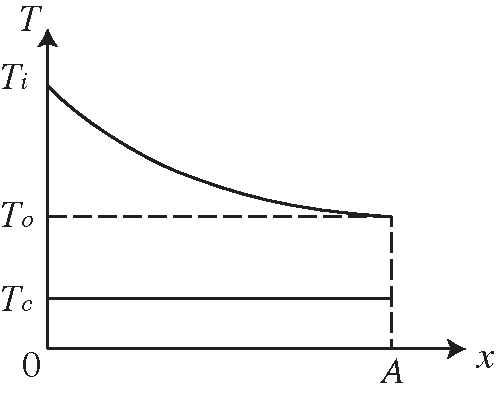
\includegraphics[width = 0.3\columnwidth]{fig/ConstTempHX}
%	\caption{Diagram of heat transfer to a constant temperature heat source}
%	\label{fig:ConstTempHX}
%\end{center}
%\end{figure}

%So
%
%\begin{equation}
%	\frac{dT}{dA}=-\frac{U}{\dot{m}c_p}(T-T_c)
%\end{equation}
%A simple Stirling engine model is used for the system. The cycle efficiency is given by \cite{Stine1985}
%
%\begin{equation}
%	\eta=\frac{T_{H}-T_{L}}{T_{H}+\text{\ensuremath{\dfrac{1-e}{k-1}}}\cdot\dfrac{T_{H}-T_{L}}{\ln\gamma}}\label{eq:eta_stirling}
%\end{equation}
%
%
%where \nomenclature{$e$}{Regeneration effectiveness of the Stirling engine}$e = (T_{R}-T_{L}) / (T_{H}-T_{L})$,\nomenclature{$T_R$}{Regenerator temperature, K}$T_{R}$ is the\emph{ }regenerator temperature, \nomenclature{$c_p$}{Heat capacity of Stirling engine working gas at constant pressure, J/(kg$\cdot$K)}\nomenclature{$c_v$}{Heat capacity of Stirling engine working gas at constant volume, J/(kg$\cdot$K)}$k=c_{p}/c_{v}$ for the working gas, $\gamma_{se}=V_{max}/V_{min}$ is the compression ratio.
%
%The heat transfer diagram is shown in Figure~\ref{fig:Heat-transfer-diagram}. Flow 1 is used for heating the hot chamber of Stirling engine, $T_{1i}$ is the inlet temperature, $T_{1o}$ is the outlet temperature. Flow 2 is used for cooling the cold chamber of Stirling engine, $T_{2i}$ is the inlet temperature, $T_{2o}$ is the outlet temperature. \nomenclature{$T_H$}{Highest temperature of expansion space, K}$T_{H}$ is the highest temperature of expansion space, \nomenclature{$T_L$}{Lowest temperature of compression space, K}$T_{L}$ is the lowest temperature of compression space.
%
%\noindent \begin{center}
%\begin{figure}[h]
%	\noindent \centering{}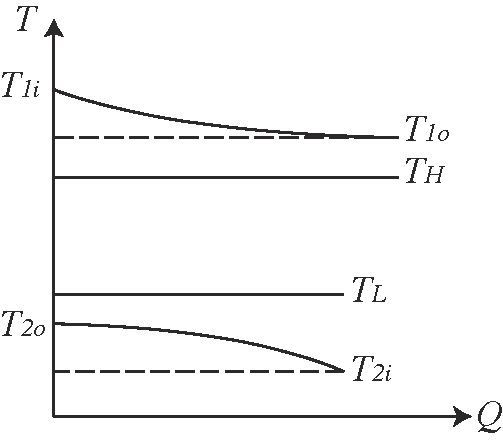
\includegraphics[width=0.4\columnwidth]{fig/StirilingHT}
%	\protect\caption{\label{fig:Heat-transfer-diagram}Heat transfer diagram of Stirling
%engine}
%\end{figure}
%
%\par\end{center}
%
%According to Equation (\ref{eq:Eq}),
%
%\begin{equation}
%	\dfrac{T_{1o}-T_{H}}{T_{1i}-T_{H}}=\exp(-\dfrac{U_{1}A_{1}}{\dot{m}_{1}c{}_{p1}})
%\end{equation}
%
%and
%
%\begin{equation}
%	\dfrac{T_{2o}-T_{L}}{T_{2i}-T_{L}}=\exp(-\dfrac{U_{2}A_{2}}{\dot{m}_{2}c_{p2}})
%\end{equation}
%
%So known $T_{1o},T_{1i},U_{1},A_{1},\dot{m}_{1},c_{p1},T_{2o},T_{2i},U_{2},A_{2},\dot{m}_{2},c_{p2}$, $T_{H}$ and $T_{L}$ can be calculated, and then $\eta$ can be obtained by using Equation (\ref{eq:eta_stirling}).
%\nomenclature{$A$}{Area, m$^2$}

For a Stirling engine, $T_{hw}$ or $T_{cw}$ can be used to substitute $T_w$ to get the relationships between $T_{i,h}$, $T_{o,h}$ and $T_{hw}$, or $T_{i,c}$, $T_{o,c}$ and $T_{cw}$ respectively.
\nomenclature[S]{$h$}{Heating fluid}
\nomenclature[S]{$c$}{Cooling fluid}
\begin{equation}
	\frac{T_{o,h}-T_{hw}}{T_{i,h}-T_{hw}}=\exp(-\frac{U_hA_h}{\dot{m}_hc_{p,h}})
	\label{Eq:T_h}
\end{equation}
\begin{equation}
	\frac{T_{o,c}-T_{cw}}{T_{i,c}-T_{cw}}=\exp(-\frac{U_cA_c}{\dot{m}_cc_{p,c}})
	\label{Eq:T_c}
\end{equation}

Heat transferred from heating fluid to Stirling engine in a cycle
\begin{equation}
	\dot{m}_hc_{p,h}(T_{i,h}-T_{o,h})/s_{se} = Q
	\label{Eq:q_h}
\end{equation}

Heat transferred from Stirling engine to cooling fluid in a cycle
\begin{equation}
	\dot{m}_cc_{p,c}(T_{o,c}-T_{i,c})/s_{se} = Q - W
	\label{Eq:q_c}
\end{equation}

%For a Stirling engine given $\dot{m}_h$, $\dot{m}_c$ and $s_{se}$, known 2 of the 6 parameters ($T_{i,h}$, $T_{o,h}$, $T_{i,c}$, $T_{o,c}$, $T_H$ and $T_L$), the rest 4 can be obtained by solving
%%Equation~\ref{Eq:T_h},~\ref{Eq:T_c},~\ref{Eq:q_h} and~\ref{Eq:q_c}
%Equation~\ref{Eq:T_h}-\ref{Eq:q_c}
%. Then $\eta$ and $P$ can be obtained by Equation~\ref{Eq:eta} and~\ref{Eq:P}. This means the performance of a given Stirling engine can be inquired by the input/output parameters of heating/cooling fluids.

\subsection{Rankine power generation system}
%The power generating system includes the turbine (steam turbine or ORC turbine) and generator.

The Rankine power generation system consists of turbine, condenser, deaerator, generator and pumps. Based on different working fluids, there are two different kinds of Rankine power generation systems, steam Rankine power generation system and organic Rankine power generation.
\subsubsection{Steam Rankine cycle}
  
  For steam Rankine cycle, deaerator is used to remove the oxygen and other non-condensable gases in the feedwater to steam generating system. Dissolved oxygen in feedwater will cause serious corrosion damage in steam generating system by forming oxides (rust) of the metal pipes. Dissolved carbon dioxide combines with water to form carbonic acid will cause further corrosion. The accumulation of the non-condensable gases will increase the heat transfer resistance, which is harmful for the heat exchangers. The extraction of the steam turbine provides heat for the deaerator.
  
  Figure~\ref{fig:Ts_Water} shows the $T$-$s$ diagram of the water circuit in the cascade system in Figure~\ref{fig:PES}. Process $2a$-$2c$-$2b$ shows the heat process in the steam turbine. (see Figure~\ref{fig:SteamTurbine_hs}) State point $2b$ and $i,2b$ have the same pressure, state point $2c$ and $i,2c$. To simplify the inner process $2a$-$2c$-$2b$ of the turbine, same isentropic efficiency of steam turbine with different loads and in different stages is assumed, which means  
  \begin{equation}
      \eta_{i,tb} =(h_{2a}-h_{2b})/(h_{2a}-h_{i,2b}) = (h_{2a}-h_{2c})/(h_{2a}-h_{i,2c})
\end{equation}
where $h_{i,2b}$ is determined by $s_{2a}$ and $p_c$; $h_{i,2c}$ is determined by $s_{2a}$ and $p_e$.

\noindent \begin{figure}[htbp]
\centering
	\begin{subfigure}[b]{0.6\columnwidth}
	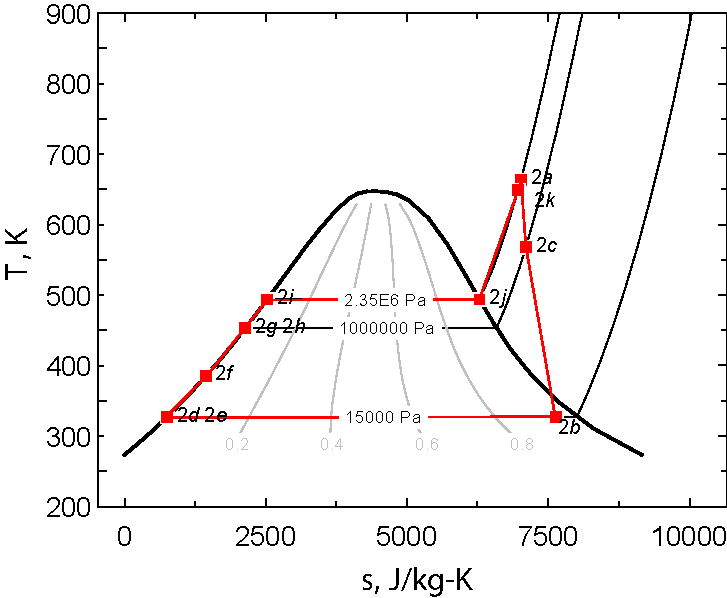
\includegraphics[width = \columnwidth]{fig/T-s_Water.pdf}
	\caption{$T$-$s$ diagram of the water circuit}\label{fig:Ts_Water}
	\end{subfigure}
	~
\begin{subfigure}[b]{0.3\columnwidth}
	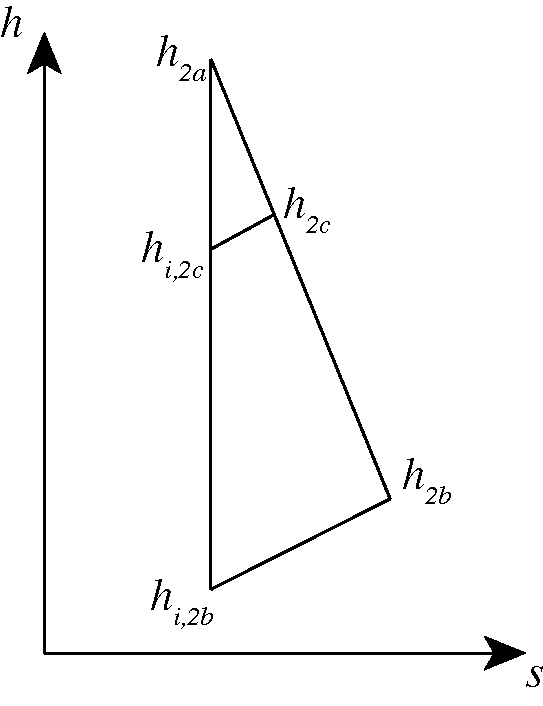
\includegraphics[width = \columnwidth]{fig/SteamTurbine_hs.pdf}
	\caption{$h$-$s$ diagram of the process $2a$-$2c$-$2b$}\label{fig:SteamTurbine_hs}
	\end{subfigure}
	
	\caption{$T$-$s$ diagram of the water circuit and $h$-$s$ diagram of the process $2a$-$2b$}\label{fig:SteamTurbine_hs_p}
\end{figure}
   
    The output power of the steam turbine
    \begin{equation}
  P_{tb}=\left(1-y\right)\dot{m}_{2}\left(h_{2a}-h_{2b}\right)+y\dot{m}_{2}\left(h_{2a}-h_{2c}\right)
  \end{equation}
  \nomenclature{$y$}{Extraction rate of steam turbine}
  
  Process $2b$-$2d$ shows the heat process in the condenser. The outlet water in the condenser is saturated water. The outlet temperature $T_{2d}$ and outlet enthalpy $h_{2d}$ are determined by the exhaust pressure of the turbine $p_c$.
  The released heat of the condenser
  \begin{equation}
      Q_{cd} = (1-y)\dot{m}_2 (h_{2b} - h_{2d})
\end{equation}
\nomenclature[S]{$cd$}{Condenser}

  State points $2c$, $2f$ and $2g$ have the same pressure ($p_e$, 1$\,\mathrm{MPa}$). The water at the outlet of the deaerator is saturated fluid, its enthalpy is determined.
  \begin{equation}
  y h_{2c} + (1-y) h_{2f} = h_{2g}
\end{equation}
\nomenclature{$p_e$}{Extraction pressure of the steam turbine, Pa}
  
  The total power of the pumps 
\begin{equation}
	P_{pu}=\left(1-y\right)\dot{m}_{2}\left(h_{2e}-h_{2d}\right)+\dot{m}_{2}\left(h_{2h}-h_{2g}\right)
\end{equation}
    \nomenclature[S]{$pu$}{Pump}
    
where $h_{2e}$ can be obtained by $\eta_{pu} = (h_{i,2e}-h{2d})/(h_{2e}-h_{2d})$, $h_{2h}$ can be obtained by $\eta_{pu} = (h_{i,2h}-h_{2g})/(h_{2h}-h_{2g})$. $h_{i,2e}$ is determined by $s_{2d}$ and $p_e$, $h_{i,2h}$ is determined by $s_{2g}$ and $p_s$.
    
The outlet water of the deaerator is saturated water ($x = 0$), so the outlet temperature $T_{2g}$ and outlet enthalpy $h_{2g}$ of the heated fluid is determined by pressure $p_{2g}$. For the deaerator, the outlet pressure equals to any of the inlet pressure.

\begin{equation}
  p_{2g} = p_{2c}
\end{equation}

    
  Heat injected in the water circuit
\begin{equation}
	    Q_2=\left(1-y\right)\dot{m}_{2}\left(h_{2f}-h_{2e}\right)+\dot{m}_{2}\left(h_{2a}-h_{2h}\right)
    \end{equation}

The efficiency of Rankine cycle can be expressed as
\begin{equation}
	\eta_{rk}=(P_{tb}-P_{pu}/\eta_{ge})/Q_{2}
\end{equation}

  \subsubsection{ORC cycle}
  
  Compared with steam Rankine cycle, ORC has the following features:
  \begin{enumerate}[label=(\arabic*)]
  \item Organic fluid has lower boiling point, and higher evaporation pressure. It is suitable for the recovery of low temperature waste heat. Besides, it has small density and specific heat capacity, the required size of turbine, pipes and heat transfer areas are small, which is beneficial for cost saving.
  \item The exhaust fluid of the turbine is dry. So without overheat, the saturated gas can be used as the main gas for the turbine. The corrosion situation caused by the impact of the droplets to the high-speed rotating blades will not happen with ORC.
  \item Organic fluid has lower sound speed than vapor, the turbine can achieve favorable aerodynamic performance with lower wheel speed. 
  \item Organic fluid has higher condensing pressure than water. It can condense under the pressure higher than the atmosphere. The system pressure can be maintained above the atmosphere pressure to prevent air leak into the system. This means a deaerator is no more necessary.
  \item Organic fluid has low freezing point, no anti-freezing treatment is required even in the cold area.
\end{enumerate}

The shapes of curves in the $T$-$s$ diagram of different fluids are different. According to the saturated vapor curve $dT/ds$ in the $T$-$s$ diagram, the working fluid can be divided into three types: $dT / ds > 0$ means dry fluid (moisture does not form when high-pressure saturated vapor expanded reversibly from a high pressure) , most of the organic fluid are dry fluids; $dT / ds < 0$ means wet fluid (moisture forms when high-pressure saturated vapor expanded reversibly from a high pressure), such as water; $dT/ds \rightarrow \pm\infty$ means isentropic fluid, such as R134a. For the high temperature high pressure dry fluid and isentropic fluid, since there is no droplets after work in the expansion turbine, no superheater is required. On the other hand, since the purpose of the ORC focuses on the recovery of low grade heat power, a superheated approach like the traditional Rankine cycle is not appropriate. 

Figure~\ref{fig:$T$-$s$_2systems} shows the $T$-$s$ diagram of steam Rankine cycle and ORC cycle. Figure~\ref{fig:ORCsystem2} shows the schematic diagram of the ORC system. For a dry fluid, the cycle can be improved by the use of a regenerator: since the fluid has not reached the two-phase state at the end of the expansion, its temperature at this point is higher than the condensing temperature. This higher temperature fluid can be used to preheat the liquid before it enters the evaporator.
A counter-current heat exchanger is thus installed between the expander outlet and the evaporator inlet. The power required from the heat source is therefore reduced and the efficiency is increased.

  \noindent \begin{figure}[htbp]
\begin{center}
	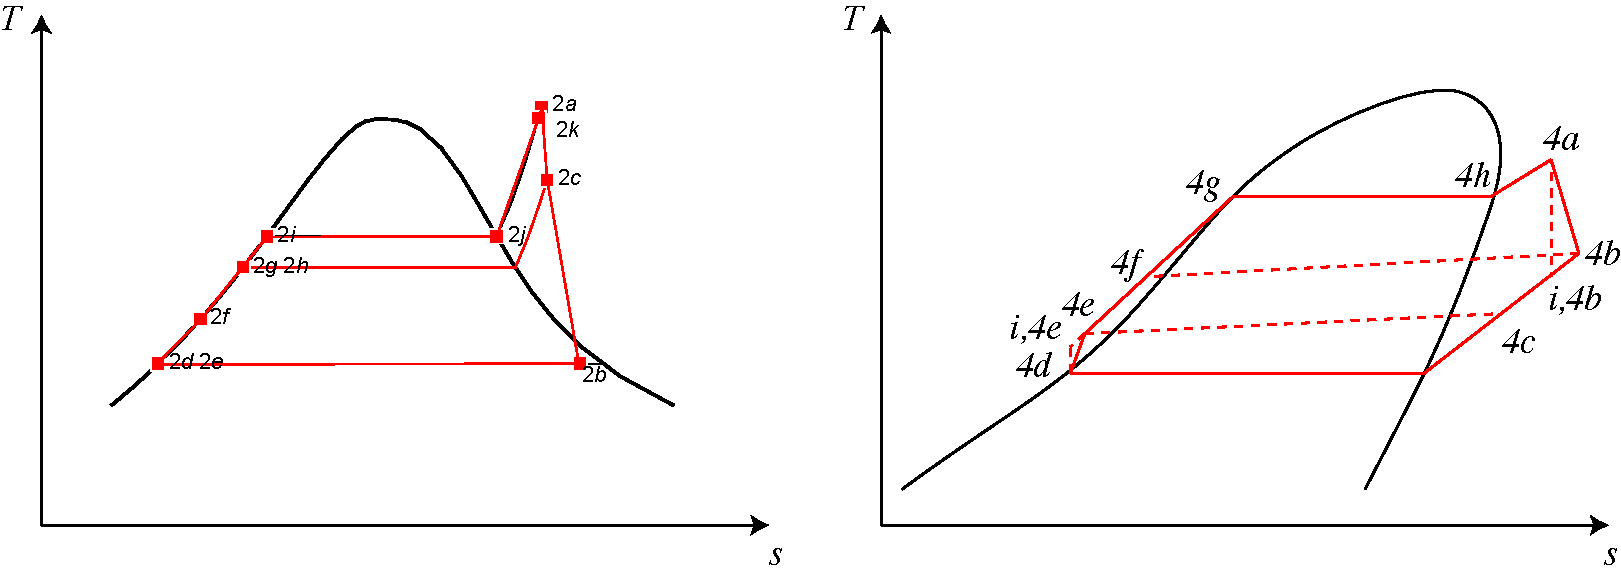
\includegraphics[width = 0.8\columnwidth]{fig/Ts.pdf}
	\caption{$T$-$s$ diagram of water and a typical organic fluid}
	\label{fig:$T$-$s$_2systems}
\end{center}
\end{figure}

\noindent \begin{figure}[htbp]
\begin{center}
	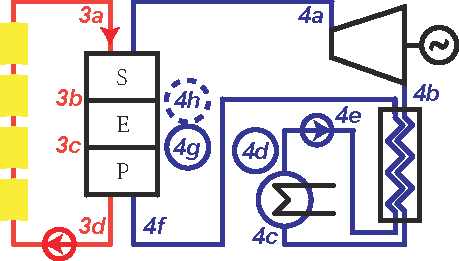
\includegraphics[width = 0.6\columnwidth]{fig/ORCsystem2.pdf}
	\caption{The schematic diagram of an ORC system with regenerator}
	\label{fig:ORCsystem2}
\end{center}
\end{figure}

The isentropic efficiency of the turbine
\begin{equation}
  \eta_{i,tb} = (h_{4a}-h_{4b})/(h_{4a}-h_{i,4b})
\end{equation}

where $h_{i,4b}$ is determined by $s_{4a}$ and $p_c$.

The output power of the turbine
\begin{equation}
  P_{tb}=\dot{m}_{4}(h_{4a}-h_{4b})
\end{equation}

Process $4c$-$4d$ shows the heat process in the condenser. The outlet fluid in the condenser is saturated liquid. The outlet temperature $T_{4d}$ and outlet enthalpy $h_{4d}$ are determined by the exhaust pressure of the turbine $p_c$.

  For the regenerator,
  \begin{equation}
      h_{4b} - h_{4c} = h_{4f} - h_{4e}
  \end{equation}
  
  The released heat of the condenser
  \begin{equation}
      Q_{cd} = \dot{m}_4 (h_{4c} - h_{4d})
\end{equation}

    The power of the pump
  \begin{equation}
	P_{pu}=\dot{m}_{4}(h_{4e}-h_{4d})
\end{equation}
    
    where $h_{4e}$ can be obtained by $\eta_{pu} = (h_{i,4e}-h{4d})/(h_{4e}-h_{4d})$. $h_{i,4e}$ is determined by $s_{4d}$ and $p_s$.
    
  Heat injected in the circuit
\begin{equation}
	    Q_4=\dot{m}_4(h_{4a}-h_{4f})
    \end{equation}

The efficiency of Rankine cycle can be expressed as
\begin{equation}
	\eta_{rk}=\dfrac{P_{tb}-P_{pu}/\eta_{ge}}{\dot{m}_4(h_{4a}-h_{4f})}
\end{equation}

%\noindent \begin{figure}[htbp]
%\begin{center}
%	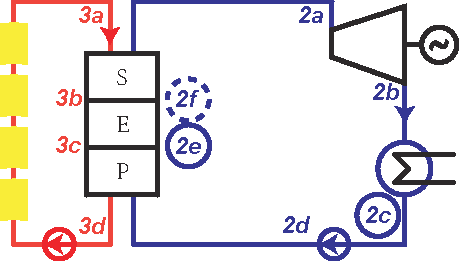
\includegraphics[width = 0.6\columnwidth]{fig/ORCsystem1.pdf}
%	\caption{The schematic diagram of an ORC system without regenerator}
%	\label{fig:ORCsystem1}
%\end{center}
%\end{figure}

%  The stream exiting the turbine was passed through a recuperator to heat the feed working fluid.


\subsubsection{Generator}
The generator is relatively independent of the cascade system and its efficiency is assumed to be a constant, 0.975.

%\subsubsection{Thermal storage system}

%\section{Steam generating system}
%\section{Steam extraction and regeneration system}
\section{Stirling engine array modeling}

Stirling engine array is used in the cascade system, Figure~\ref{fig:Layout of Stirling engines} shows the layout of the Stirling engine array. Each Stirling engine in the Stirling engine array has the identical parameters: $U_{se,1}=$30$\,\mathrm{W/(m^2\cdot{}K)}$, $U_{se,2}=$150$\,\mathrm{W/(m^2\cdot{}K)}$, $A_{se,1}=$6$\,\mathrm{m^2}$, $A_{se,2}=$6$\,\mathrm{m^2}$, $k_{se}=$1.4, $\gamma_{se}=$3.375, $n_g=$7.84$\times$10$^{-2}\,\mathrm{mol}$, $s_{se}=$10$\,\mathrm{s^{-1}}$.

\noindent \begin{figure}[htbp]
\begin{center}
	\includegraphics[width = 0.6\columnwidth]{fig/stirlingEngineArray.pdf}
	\caption{Layout of Stirling engines}
	\label{fig:Layout of Stirling engines}
\end{center}
\end{figure}

Depending on the direction of heating and cooling flows, there are two possible flow types: parallel flow and counterflow. 
Figure~\ref{fig:twoFlowTypes} and 
Figure~\ref{fig:CounterFlow} show the heat transfer diagrams of the two flow types.
\nomenclature{$n_1$}{Number of columns of the Stirling engine array} $n_1$ is chosen to be 10 and can be optimized later.

\noindent \begin{figure}[htbp]
\centering
	\begin{subfigure}[b]{0.4\columnwidth}
	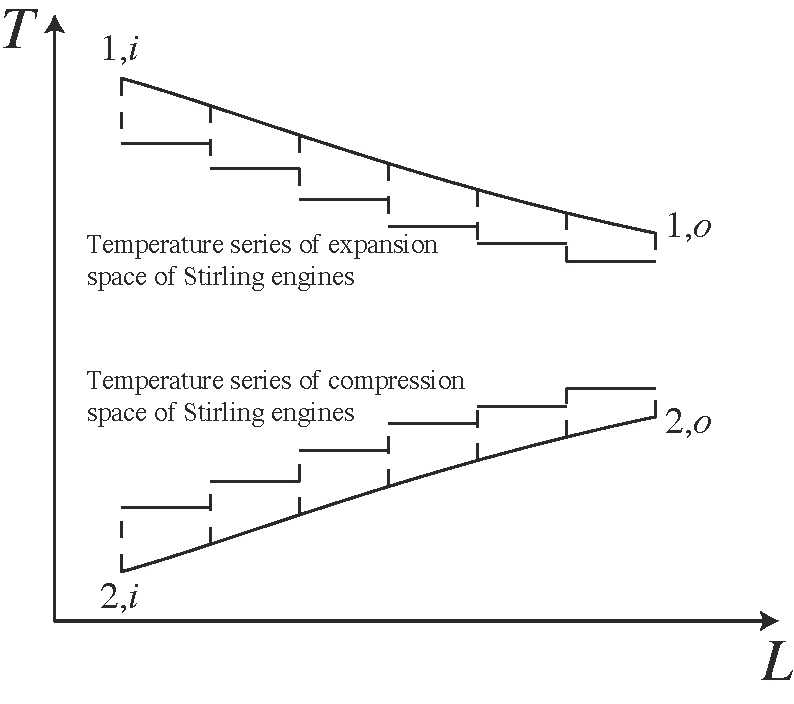
\includegraphics[width = \columnwidth]{fig/HeatTransfer_Parallel.pdf}
	\caption{Parallel flow}\label{fig:ParallelFlow}
	\end{subfigure}
	~
\begin{subfigure}[b]{0.4\columnwidth}
	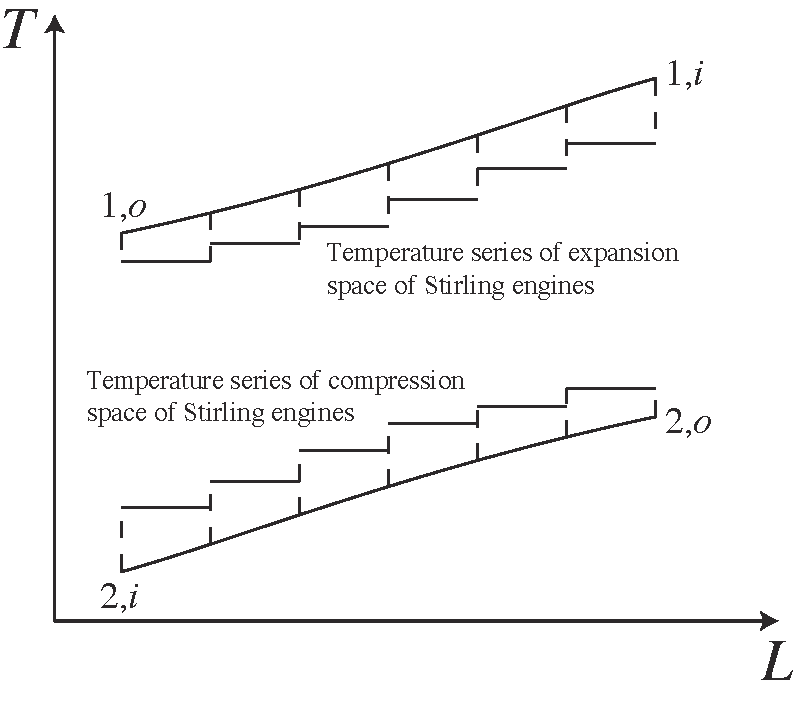
\includegraphics[width = \columnwidth]{fig/HeatTransfer_Counter.pdf}
	\caption{Counterflow}\label{fig:CounterFlow}
	\end{subfigure}
	\caption{Heat transfer diagram of parallel flow and counterflow}
	\label{fig:twoFlowTypes}
\end{figure}

%\noindent \begin{figure}[htbp]
%\begin{center}
%	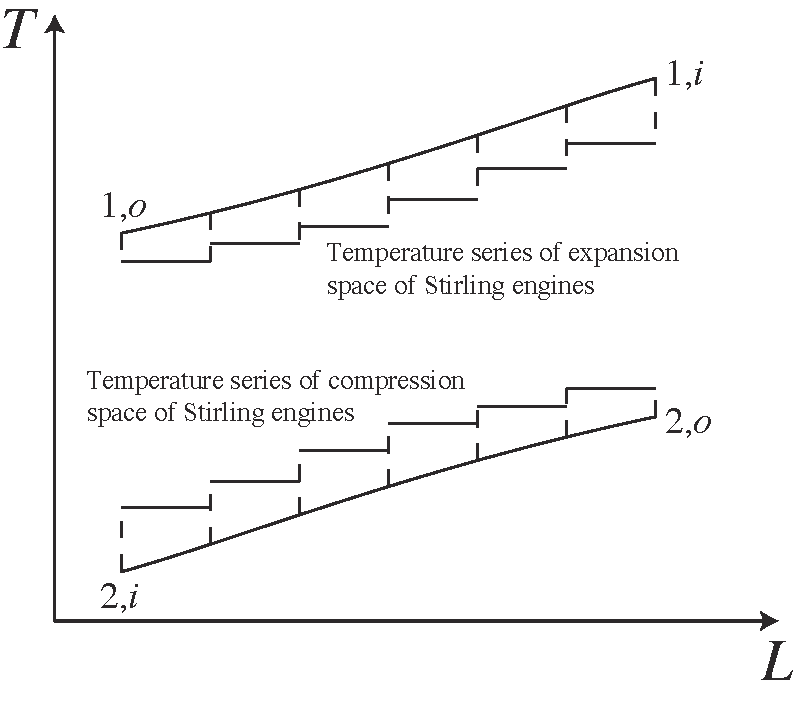
\includegraphics[width = 0.7\columnwidth]{fig/HeatTransfer_Counter}
%	\caption{Heat transfer diagram of counterflow}
%	\label{fig:CounterFlow}
%\end{center}
%\end{figure}

In Figure~\ref{fig:Layout of Stirling engines}, $T_{1,i,1}=T_{1,i},\dot{m}_{1,r}=\dot{m}_{1}/n_{2}$. For $x$ from $1$ to $n_1-1$, where $x$ is the column number of Stirling engines, $T_{1,i,x+1}=T_{1,o,x},T_{2,i,x+1}=T_{2,o,x}$.
\nomenclature{$n_1$}{Number of columns of the Stirling engine array}
%\nomenclature{$\dot{m}_{1}$}{Total mass flow rate of air, kg/s}

Assume that the positive flow direction is to the right, for parallel flow, $T_{2,i,1}=T_{2,i}$, $\dot{m}_{2,r}=\dot{m}_{2}/n_{2}$; for counterflow, $T_{2,o,n_1}=T_{2,i}$, $\dot{m}_{2,r}=-\dot{m}_{2}/n_{2}$.
\nomenclature{$n_2$}{Number of rows of the Stirling engine array}
\nomenclature{$\dot{m}$}{Mass flow rate, kg$\cdot$s$^{-1}$}

%\begin{equation}
%	T_{2,i,1}=T_{2,i}\label{eq:T_2_i_1}
%\end{equation}
%\begin{equation}
%	\dot{m}_{2,r}=\dot{m}_{2}/n_{2}
%\end{equation}
%\nomenclature{$\dot{m}_{2,r}$}{Mass flow rate of water in each row of Stirling engine array, kg/s}
%\nomenclature{$\dot{m}_{2}$}{Total mass flow rate of water, kg/s}

%for counterflow,
%
%\begin{equation}
%	T_{2,o,n_1}=T_{2,i}\label{eq:T_2_o_n1}
%\end{equation}
%\begin{equation}
%	\dot{m}_{2,r}=-\dot{m}_{2}/n_{2}
%\end{equation}

Assume linear temperature profile across the regenerator, the mean effective temperature $T_{R,x}=\dfrac{T_{H,x}-T_{L,x}}{\ln(T_{H,x}/T_{L,x})}$~\cite{Der2007,Cavazzuti2012}, and the symmetrical regenerator behaviour assumption $e_{x}=\dfrac{T_{R,x}-T_{L,x}}{T_{H,x}-T_{L,x}}$~\cite{Formosa2010,Juhasz2010}. For a Stirling engine in column $x$\nomenclature[S]{$x$}{Stirling engine in column $x$}, $x$ from $1$ to $n_1$, according to Equation~(\ref{eq:T_H}) and Equation~(\ref{eq:T_L}),

\begin{equation}
	T_{hw,x}=T_{1,i,x}-\dfrac{T_{1,i,x}-T_{1,o,x}}{1-\exp(-\dfrac{U_{se,1}A_{se,1}}{\dot{m}_{1,r}c_{p,1,x}})}\label{eq:T_H_x}
\end{equation}


\begin{equation}
	T_{cw,x}=T_{2,i,x}-\dfrac{T_{2,i,x}-T_{2,o,x}}{1-\exp(-\dfrac{U_{se,2}A_{se,2}}{\dot{m}_{2,r}c_{p,2,x}})}\label{eq:T_L_x}
\end{equation}

The power of each Stirling engine in column $x$ can be written as 
\begin{equation}
  P_{se,x} = W_{th,x}-W_{pd,x}-W_{fs,x}
\end{equation}

The efficiency of each Stirling engine in column $x$ can be written as 
\begin{equation}
  \eta_{se,x} = \dfrac{W_{th,x}-W_{pd,x}-W_{fs,x}}{Q_{th,x}+Q_{id,x}+Q_{sc,x}}
\end{equation}

%$\eta_{se,x}=\dfrac{T_{H,x}-T_{L,x}}{T_{H,x}+\dfrac{1-e_{x}}{k-1}\cdot\dfrac{T_{H,x}-T_{L,x}}{\ln\gamma_{se}}}\label{eq:eta_striling_x}$, where $e_{x}=\dfrac{T_{R,x}-T_{L,x}}{T_{H,x}-T_{L,x}}$~\cite{Stine1985,Juhasz2010} and $T_{R,x}=\dfrac{T_{H,x}-T_{L,x}}{\ln(T_{H,x}/T_{L,x})}$~\cite{Der2007,Cavazzuti2012}.

%\begin{equation}
%	\eta_{se,x}=\dfrac{T_{H,x}-T_{L,x}}{T_{H,x}+\dfrac{1-e_{x}}{k-1}\cdot\dfrac{T_{H,x}-T_{L,x}}{\ln\gamma_{se}}}\label{eq:eta_striling_x}
%\end{equation}

For energy balance,
\begin{equation}
	\dot{m}_{1,r}(h_{1,i,x}-h_{1,o,x})(1-\eta_{se,x})=\dot{m}_{2,r}(h_{2,o,x}-h_{2,i,x})
\end{equation}

%And in each Stirling cycle, the heat absorbed by the working gas is
%\begin{equation}
%\begin{split}
%	n_gR(T_{H,x}\ln\gamma_{se}+\dfrac{1-e_{x}}{k-1}(T_{H,x}-T_{L,x}))=\dot{m}_{1,r}(h_{1,i,x}-h_{1,o,x})/s_{se}
%\end{split}
%\end{equation}

By using equations in Section~\ref{sec:StirlingEngineModel} and the energy balance equations, key parameters of the Stirling engine array can be obtained. 

The efficiency of the Stirling engine array 
\begin{equation}
  \eta_{sea}=1-\dfrac{\dot{m}_{2}(h_{2,o,n_1}-h_{2,i,1})}{\dot{m}_{1}(h_{1,i,1}-h_{1,o,n_1})}
\end{equation}

The output power of each Stirling engine in column $x$
\begin{equation}
  P_{se,x}=\dot{m}_{1,r}(h_{1,i,x}-h_{1,o,x})\eta_{se,x}
\end{equation}

The output power of the Stirling engine array
\begin{equation}
  P_{sea}=\eta_{sea}\dot{m}_{1}(h_{1,i,1}-h_{1,o,n_1})
\end{equation}

\section{Steam generating system modeling}
The steam generating system can be divided into preheater, evaporator and superheater, they are collectively referred to as PES. They are all heat exchangers. It is assumed that, in these heat exchangers, the pressure of the fluid does not change significantly. It can be assumed to be equal to the pressure of the inlet pressure of the turbine. Besides, these heat exchangers do not exchange heat with the environment.
To clearly understand the modeling process of these heat exchangers, an example of steam generating system as shown in Figure~\ref{fig:PES} is used for explanation. Figure~\ref{fig:PES_TQ} shows the $T$-$Q$ diagram of the heat transfer process. State points of different fluids are marked on the sketch. The number indicates the type of the fluid, the letter indicates the state point of the fluid. A state point with solid circle indicates saturated liquid state ($x = 0$), and with dotted circle indicates saturated gas state ($x = 1$).
\nomenclature{$x$}{Dryness fraction}

%State points of different fluids are marked on the sketch. The number indicates the type of the fluid, the letter indicates the state point of the fluid. State points with solid circle indicate saturated liquid states ($x = 0$\nomenclature{$x$}{Dryness fraction}), and with dotted circle indicates saturated gas states ($x = 1$).

\noindent \begin{figure}[!ht]
\begin{center}
	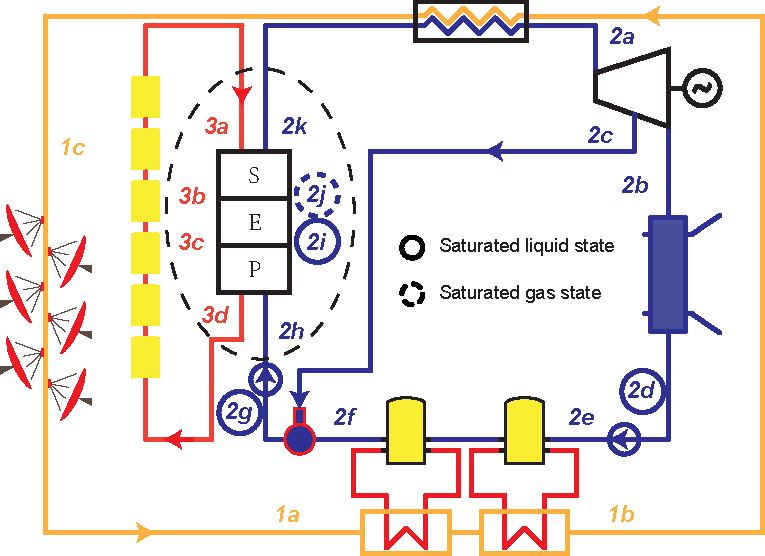
\includegraphics[width = 0.8\columnwidth]{fig/PES}
	\caption{An example of steam generating system in a cascade system}
	\label{fig:PES}
\end{center}
\end{figure}

\noindent \begin{figure}[htbp]
\begin{center}
	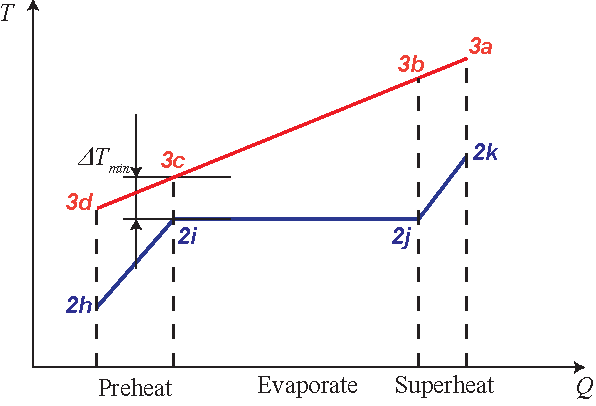
\includegraphics[width = 0.8\columnwidth]{fig/PES_TQ}
	\caption{The steam generating process}
	\label{fig:PES_TQ}
\end{center}
\end{figure}

The modeling process of PES is the process of solving the unknown states of the state points. Notice that, the pressure of the fluids keeps constant in the heat transfer process. For an unsaturated state, known the temperature or enthalpy, the state is determined. This means, the temperature can be obtained by the enthalpy, and vice versa. For a saturated state, known the dryness ($x$) of the fluid, the state is determined.

For a typical PES modeling process as shown in Figure~\ref{fig:PES}, $\dot{m}_2$, state $2h$ and state $2k$ are determined by the parameters of the turbine. State $3a$ is determined by the design parameters. State $2i$ and state $2j$ are determined by their dryness values. 

\begin{enumerate}[label=(\arabic*)]
  \item \emph{Preheater}
  
  The outlet of the heated fluid is saturated liquid ($x = 0$), so the outlet temperature $T_{2i}$ and outlet enthalpy $h_{2i}$ of the heated fluid are determined by the main pressure of the turbine, $p_s$.
  \begin{equation}
  \dot{m}_3 (h_{3c}-h_{3d})=\dot{m}_2 (h_{2i} - h_{2h})
  \label{eq:preheater}
\end{equation}

  \item \emph{Evaporator}
  
  The outlet of the heated fluid is saturated gas ($x = 1$), so the outlet temperature $T_{2j}$ and outlet enthalpy $h_{2j}$ of the heated fluid are determined by the main pressure of the turbine, $p_s$.
  \begin{equation}
  \dot{m}_3 (h_{3b}-h_{3c})=\dot{m}_2 (h_{2j} - h_{2i})
  \label{eq:evaporator}
\end{equation}
	It has to be mentioned that, state $3c$ is determined by $T_{3c}$, which equals to $T_{2i} + \Delta T_{min}$. ($T_{3c} = T_{2i} + \Delta T_{min}$)
  
  \item \emph{Superheater}
  
  For the energy balance,
  \begin{equation}
  \dot{m}_3 (h_{3a}-h_{3b})=\dot{m}_2 (h_{2k} - h_{2j})
  \label{eq:superheater}
\end{equation}
	  
\end{enumerate}

By solving the equations~(\ref{eq:preheater}) to~(\ref{eq:superheater}), $\dot{m}_3$, state $3b$ and $3d$ can be obtained.

\section{System modeling}

%\subsection{Stream}
Different components are connected to form a system by their interfaces (inlets and outlets). These interfaces are interacted with each other by "streams". For example, the steam turbine in Figure~\ref{fig:PES} is connected with the deaerator by a steam stream. This steam stream has its own properties such as fluid type, mass flow rate, temperature, pressure and so on.
"Steams" are defined as objects in the modeling language -- MATLAB. Appendix~\ref{cha:MATLAB_SOURCECODE} shows the source code of the definition of the class -- \textbf{Stream}.

Some properties, \textbf{T}, \textbf{q\_m} and \textbf{p}, of \textbf{Stream} are also objects. They belong to the classes \textbf{Temperature}, \textbf{Massflow} and \textbf{Pressure} separately.

Given the inherent properties of a \textbf{Stream}, its dependent properties, mass specific enthalpy (\textbf{h}), mass specific entropy (\textbf{s}) and pressure (\textbf{p}), can be obtained.

If the stream is a single phase stream, its dryness does not exist. Its dependent properties ($h$, $s$, $c_p$) can be obtained by its temperature ($T$) and pressure ($p$) by calling the open source MATALB wrapper CoolProp. If the stream is a two-phase stream, $0 \leqslant x \leqslant 1$. Its dependent properties ($h$, $s$, $c_p$) can be obtained by its pressure ($p$) and dryness ($x$). The reason of choosing pressure ($p$) instead of temperature ($T$) as the input value is that it is easier to be determined.

A \textbf{stream} can be used to record a state point since it contains all the information for a state point. Streams are defined in a system for component connection and system calculation. Different components are connected by streams to form a system. The Streams are passed as parameters to the components, completing the calculation of the methods in the components.

%\subsection{System connection}
Components are connected each other by streams. Their inlets and outlets are used as interfaces for connection. 
Two interfaces are connected together by being assigned the same stream.

%\subsection{System initialization}
Systems are initialized by given parameters (design parameters). These parameters are assigned to corresponding properties of the streams and thus affect the state of the related components.

%\subsection{System calculation}
For system calculation, it has to be mentioned that, some parameters of a component are related with other components. 
In such situations, guess values are used for the calculation methods in the components.
The guess values are set to be the properties of some streams. Each of these streams is assigned to two components (evaporator and superheater). These streams are assigned to corresponding components to accomplish the calculation methods in the components. These calculation methods will return solutions for the stream parameters. Then the parameters will be compared with the guess values for verification. If the differences between guess values and the calculated parameters are within permissible error, the guess values are accepted; otherwise, the guess values will be iteratively readjusted according to the Runge-Kutta method until accepted.

For example, the mass flow rate of oil of the evaporator ($\dot{m}_3$) is related with the superheater in a system as described in Figure~\ref{fig:CascadeSystem1}.
A guess value of $\dot{m}_3$, $\dot{m}_{3,g}$, is required to determine it. $\dot{m}_{3,g}$ is assigned to the evaporator oil stream. This stream is assigned to both evaporator and superheater. In \textbf{evaporator}, the method \textbf{get\_T\_3b} will change the temperature of the stream ($T_{3b}$) from the default value. 
In \textbf{superheater}, the method \textbf{get\_q\_m\_3} will return a solution of $\dot{m}_3$, $\dot{m}_{3,s}$, for verification. If $\left|\dot{m}_{3,g} - \dot{m}_{3,s}\right|$ is less than permissible error ($10^{-4}$), then $\dot{m}_{3,g}$ is accepted as the value of $\dot{m}_{3}$; otherwise, $\dot{m}_{3,g}$ will be iteratively readjusted according to the Runge-Kutta method until $\left|\dot{m}_{3,g} - \dot{m}_{3,s}\right| < 10^{-4}$.

\section{Conclusion}

This chapter presents the modeling method of the cascade system and introduces the modeling of some key components and subsystems in detail. The component models were developed in MATLAB by using object-oriented method. Bottom-up design method is applied for system development. Models of the components of a system are developed first according to their mechanism characteristics, and the system model is established by these component models. A MATLAB class \textbf{Stream} is created for component connection. The components' inlets and outlets are used as interfaces for connection. 
Two interfaces are connected together by being assigned the same stream.
The calculation process related with different components is also briefly introduced in this chapter.

Due to the encapsulation, composition and polymorphism of the object-oriented language, the system model has some advantages such as easy to establish, convenient to replace a component and clearly check the performance of specific components.

The key component models in the cascade system can be validated experimentally or be compared with the classic models. The validation of Stirling engine model shows that the proposed model has much better agreement with the experimental results than previous classic thermal models at various rotation speeds and mean effective pressures.